% !TeX spellcheck = fr_FR
\chapter{Digital Communities in Practice}

\section{Discord}
Essentially now synonymous with gaming messengers, Discord is an instant messenger that supports chat, calls, and screen sharing. It was launched on May 13, 2015, to support the mobile MOBA game Fates Forever.  

It is a messenger program primarily used by gamers who enjoy online games. Based on excellent performance and convenience, it has surpassed mainstream messengers that gamers had used in the past and has now established itself as a major application. Discord’s server locations apply only to voice chat. All text chat traffic is processed through data centers located on the U.S. East Coast.  

It is an Electron-based program developed with early support and funding from the startup incubator YouWeb's 9+ Incubator, with later investments from Benchmark Capital and Tencent. The developers sought to combine only the advantages of VoIP software such as Skype, Slack, and TeamSpeak, and to create VoIP software with low latency. It became popular among esports and LAN tournament gamers. As a result, by the first half of 2022, it was announced that Discord had more than 390 million users worldwide, with approximately 150 million logging in at least once a month. Currently, it is widely known through streamers on Twitch and elsewhere, and in Korea, it is mainly used by streamers, online broadcasters, and various gaming communities. The company Discord Inc. was founded by Jason Citron, who had previously operated another mobile messenger called OpenFeint. He announced that Discord would be run as an independent company separate from OpenFeint. In January 2016, OpenFeint invested 20 million USD.  

In the early days, Discord was little more than a Slack imitation, supporting only simple voice and text chat. However, unlike Slack—which was essentially business-oriented, with most features behind a paywall and focused on productivity—Discord targeted gamers and general users. By providing intuitive and game-friendly features such as simple and fast voice chat and overlays, it succeeded in differentiating itself.  

Discord also supports an API that allows the creation of bots, such as chat or music bots, providing convenient functions such as server management and music playback. Its success also lies in having activated the user community from the very beginning and actively accepting feedback. In this way, it drew together fragmented gaming communities onto Discord.  

\begin{figure}[tbph!]
	\centering
	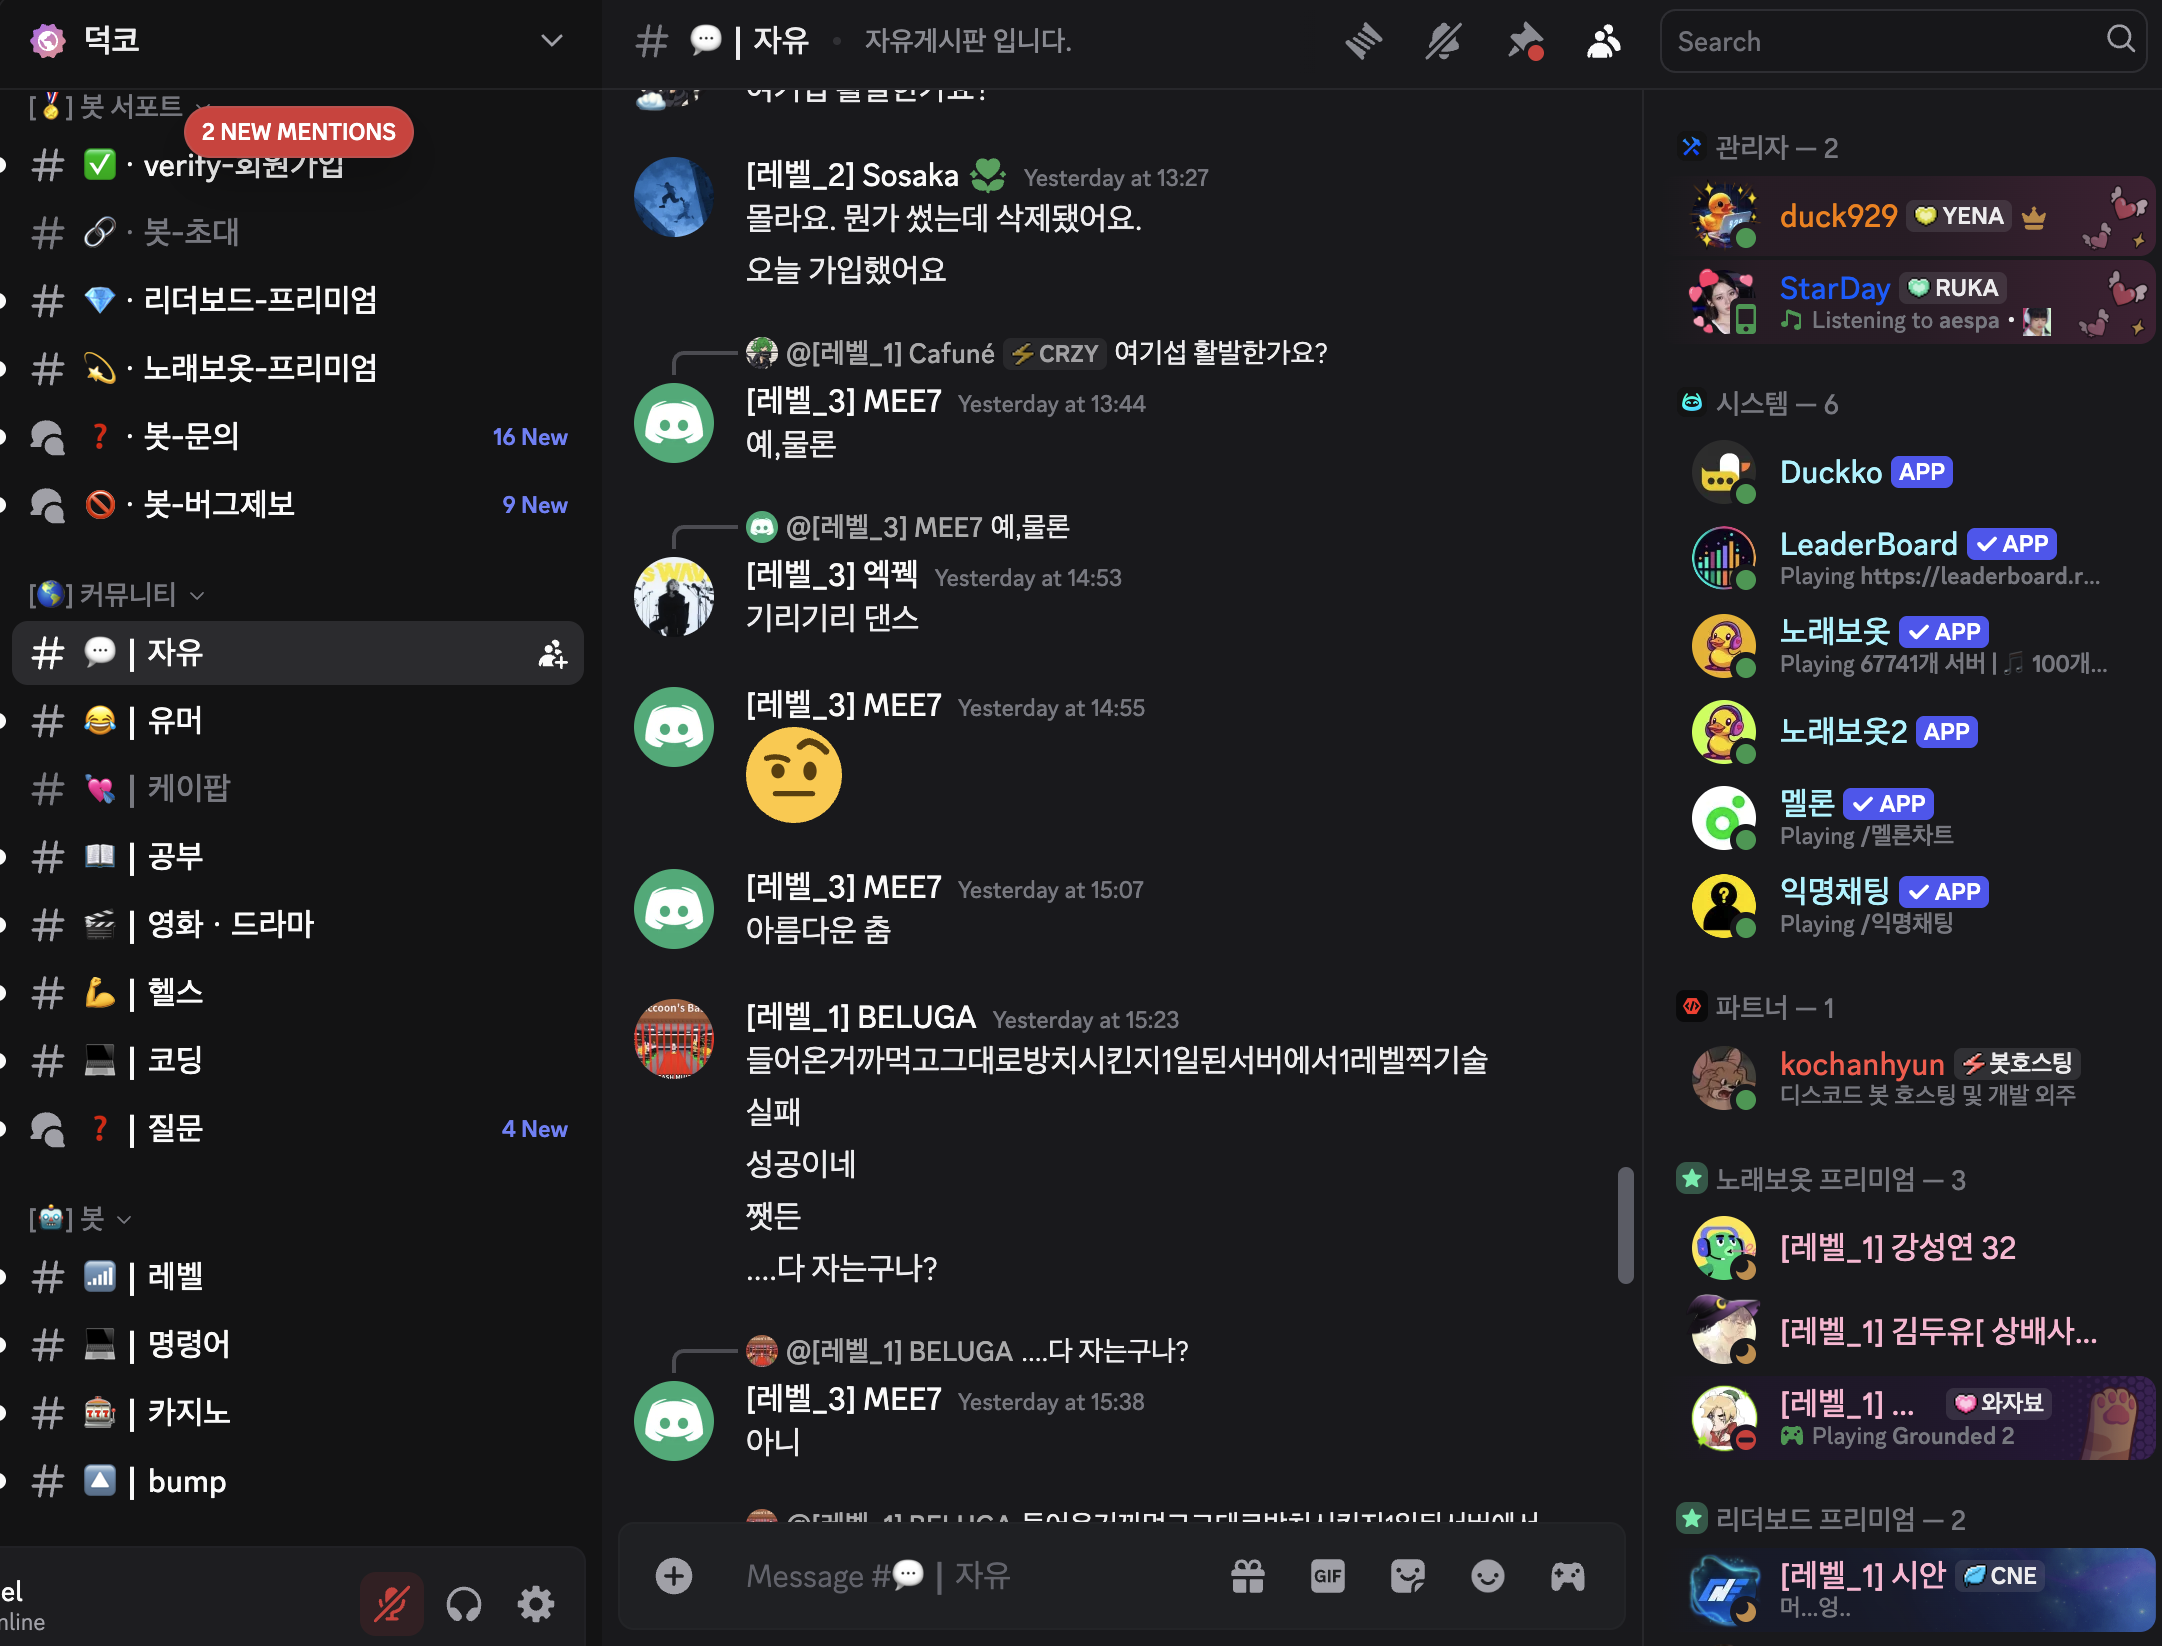
\includegraphics[width=0.7\linewidth]{template/images/chap4/discord.png}
	\caption[Discord]{Discord}
	\label{fig:image}
\end{figure}

\section{Kakaotalk Open Chat}
Open chat rooms (also called “Open KakaoTalk rooms”) refer to open chat communities created within KakaoTalk.  

Open chat rooms are created for hobbies, socializing, exchanging information, or studying. Families or friends may also create them to stay in touch, while workplaces may use them to issue work instructions. Some also exist in the form of paid sharing or paid group chatrooms where information is sold.  

They are often confused with group chats. Group chats are created by inviting registered friends in KakaoTalk, while open chat rooms can be accessed through a link. Unlike group chats, open chat rooms can be searched on social networks, and the host may require a password to join. Open chat rooms also have an administrator system that allows the host to appoint up to 10 sub-admins. This enables changing the host or expelling members.  

In short, a group chat can be seen as a gathering of acquaintances, while an open chat room can be seen as a completely open square. It is, literally, “open chat.”  

Open chat shares the strengths of messenger-type social networks. Multiple people can communicate simultaneously, and even if one does not participate in real time, they can easily catch up through saved messages. As long as one is connected, the participants and chat history remain.  

It also supports communication in multiple forms, such as file sharing, voice messages, and group calls. Depending on linked apps, it can even support money transfers and gifting. Since it is primarily mobile-based, access and participation are relatively free.  

\begin{figure}[tbph!]
	\centering
	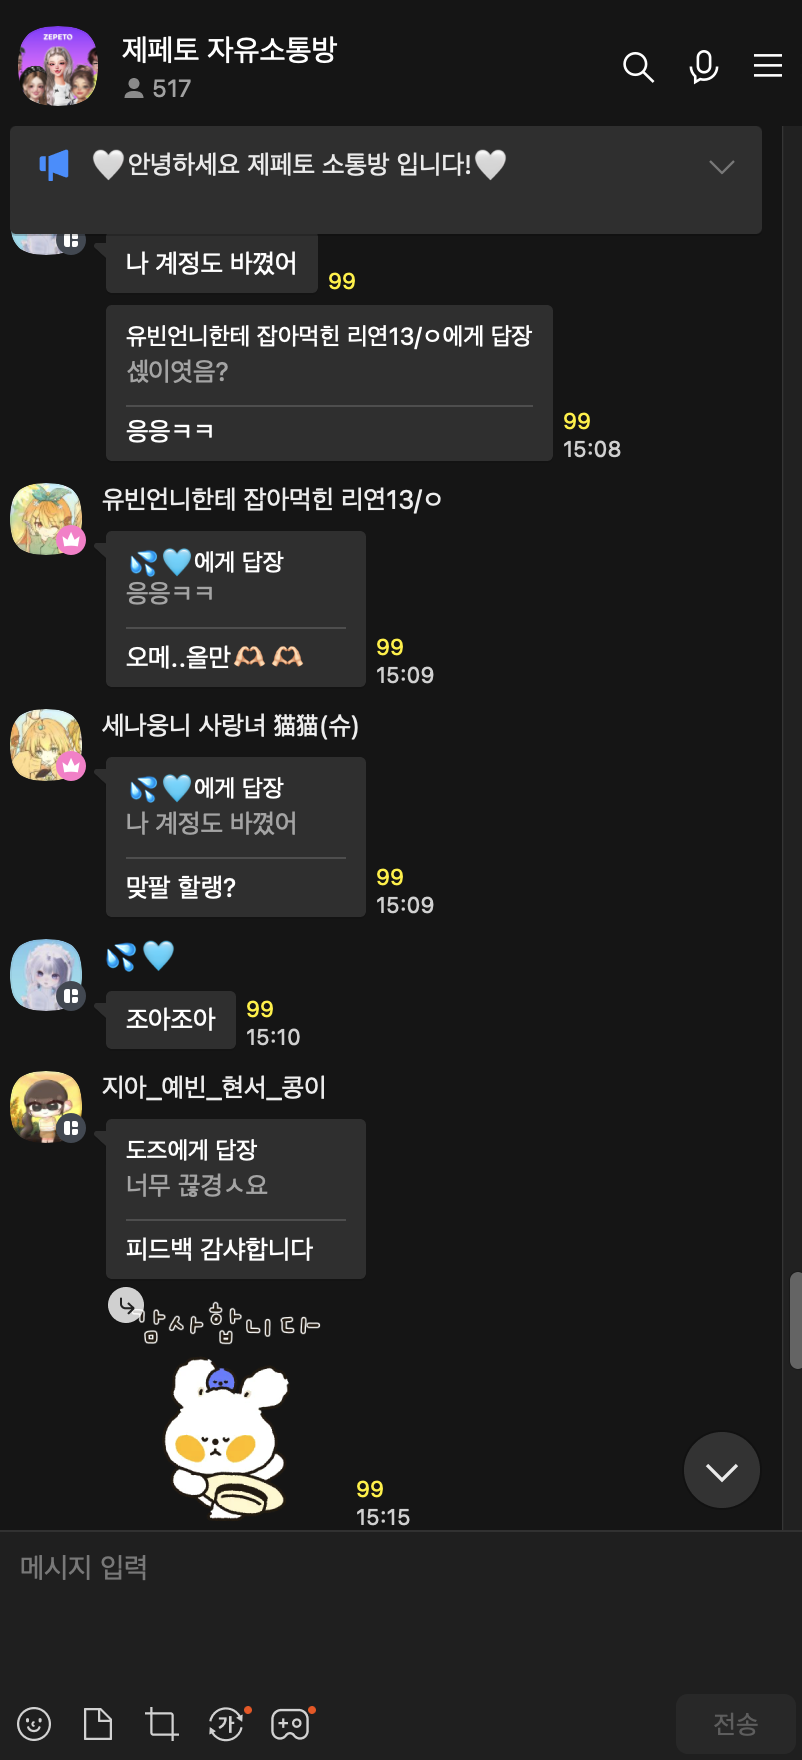
\includegraphics[width=0.3\linewidth]{template/images/chap4/kakaotalk.png}
	\caption[Kakaotalk]{Kakaotalk}
	\label{fig:image}
\end{figure}

\section{ZEPETO, Enjoy?}
ZEPETO, operated by NAVER Z, is an augmented reality (AR) avatar service and one of Korea’s representative metaverse platforms. Launched in 2018, ZEPETO uses facial recognition, AR, and 3D technology to create “3D avatars” that allow users to communicate with others and experience diverse virtual environments.  

Through AI-based facial recognition technology, ZEPETO enables the creation of a 3D AR avatar as “another self” to communicate with acquaintances and friends in virtual space. Within two months of its launch, global app downloads surpassed 3 million, and within about two years, the number of registered users exceeded 340 million. Over 90\% of these users are overseas.  

ZEPETO has also actively partnered with well-known brands such as Sanrio Characters and Snoopy, providing various content to increase popularity. Fashion companies such as Gucci, Nike, and FILA have collaborated with ZEPETO to create and sell digital goods.  

After its spinoff, ZEPETO focused on building its own avatar platform ecosystem and expanding globally. It has established “ZEPETO World,” a creator platform where users can directly design and sell items, including clothing. It is available on both mobile and PC.  

\begin{figure}
    \centering
    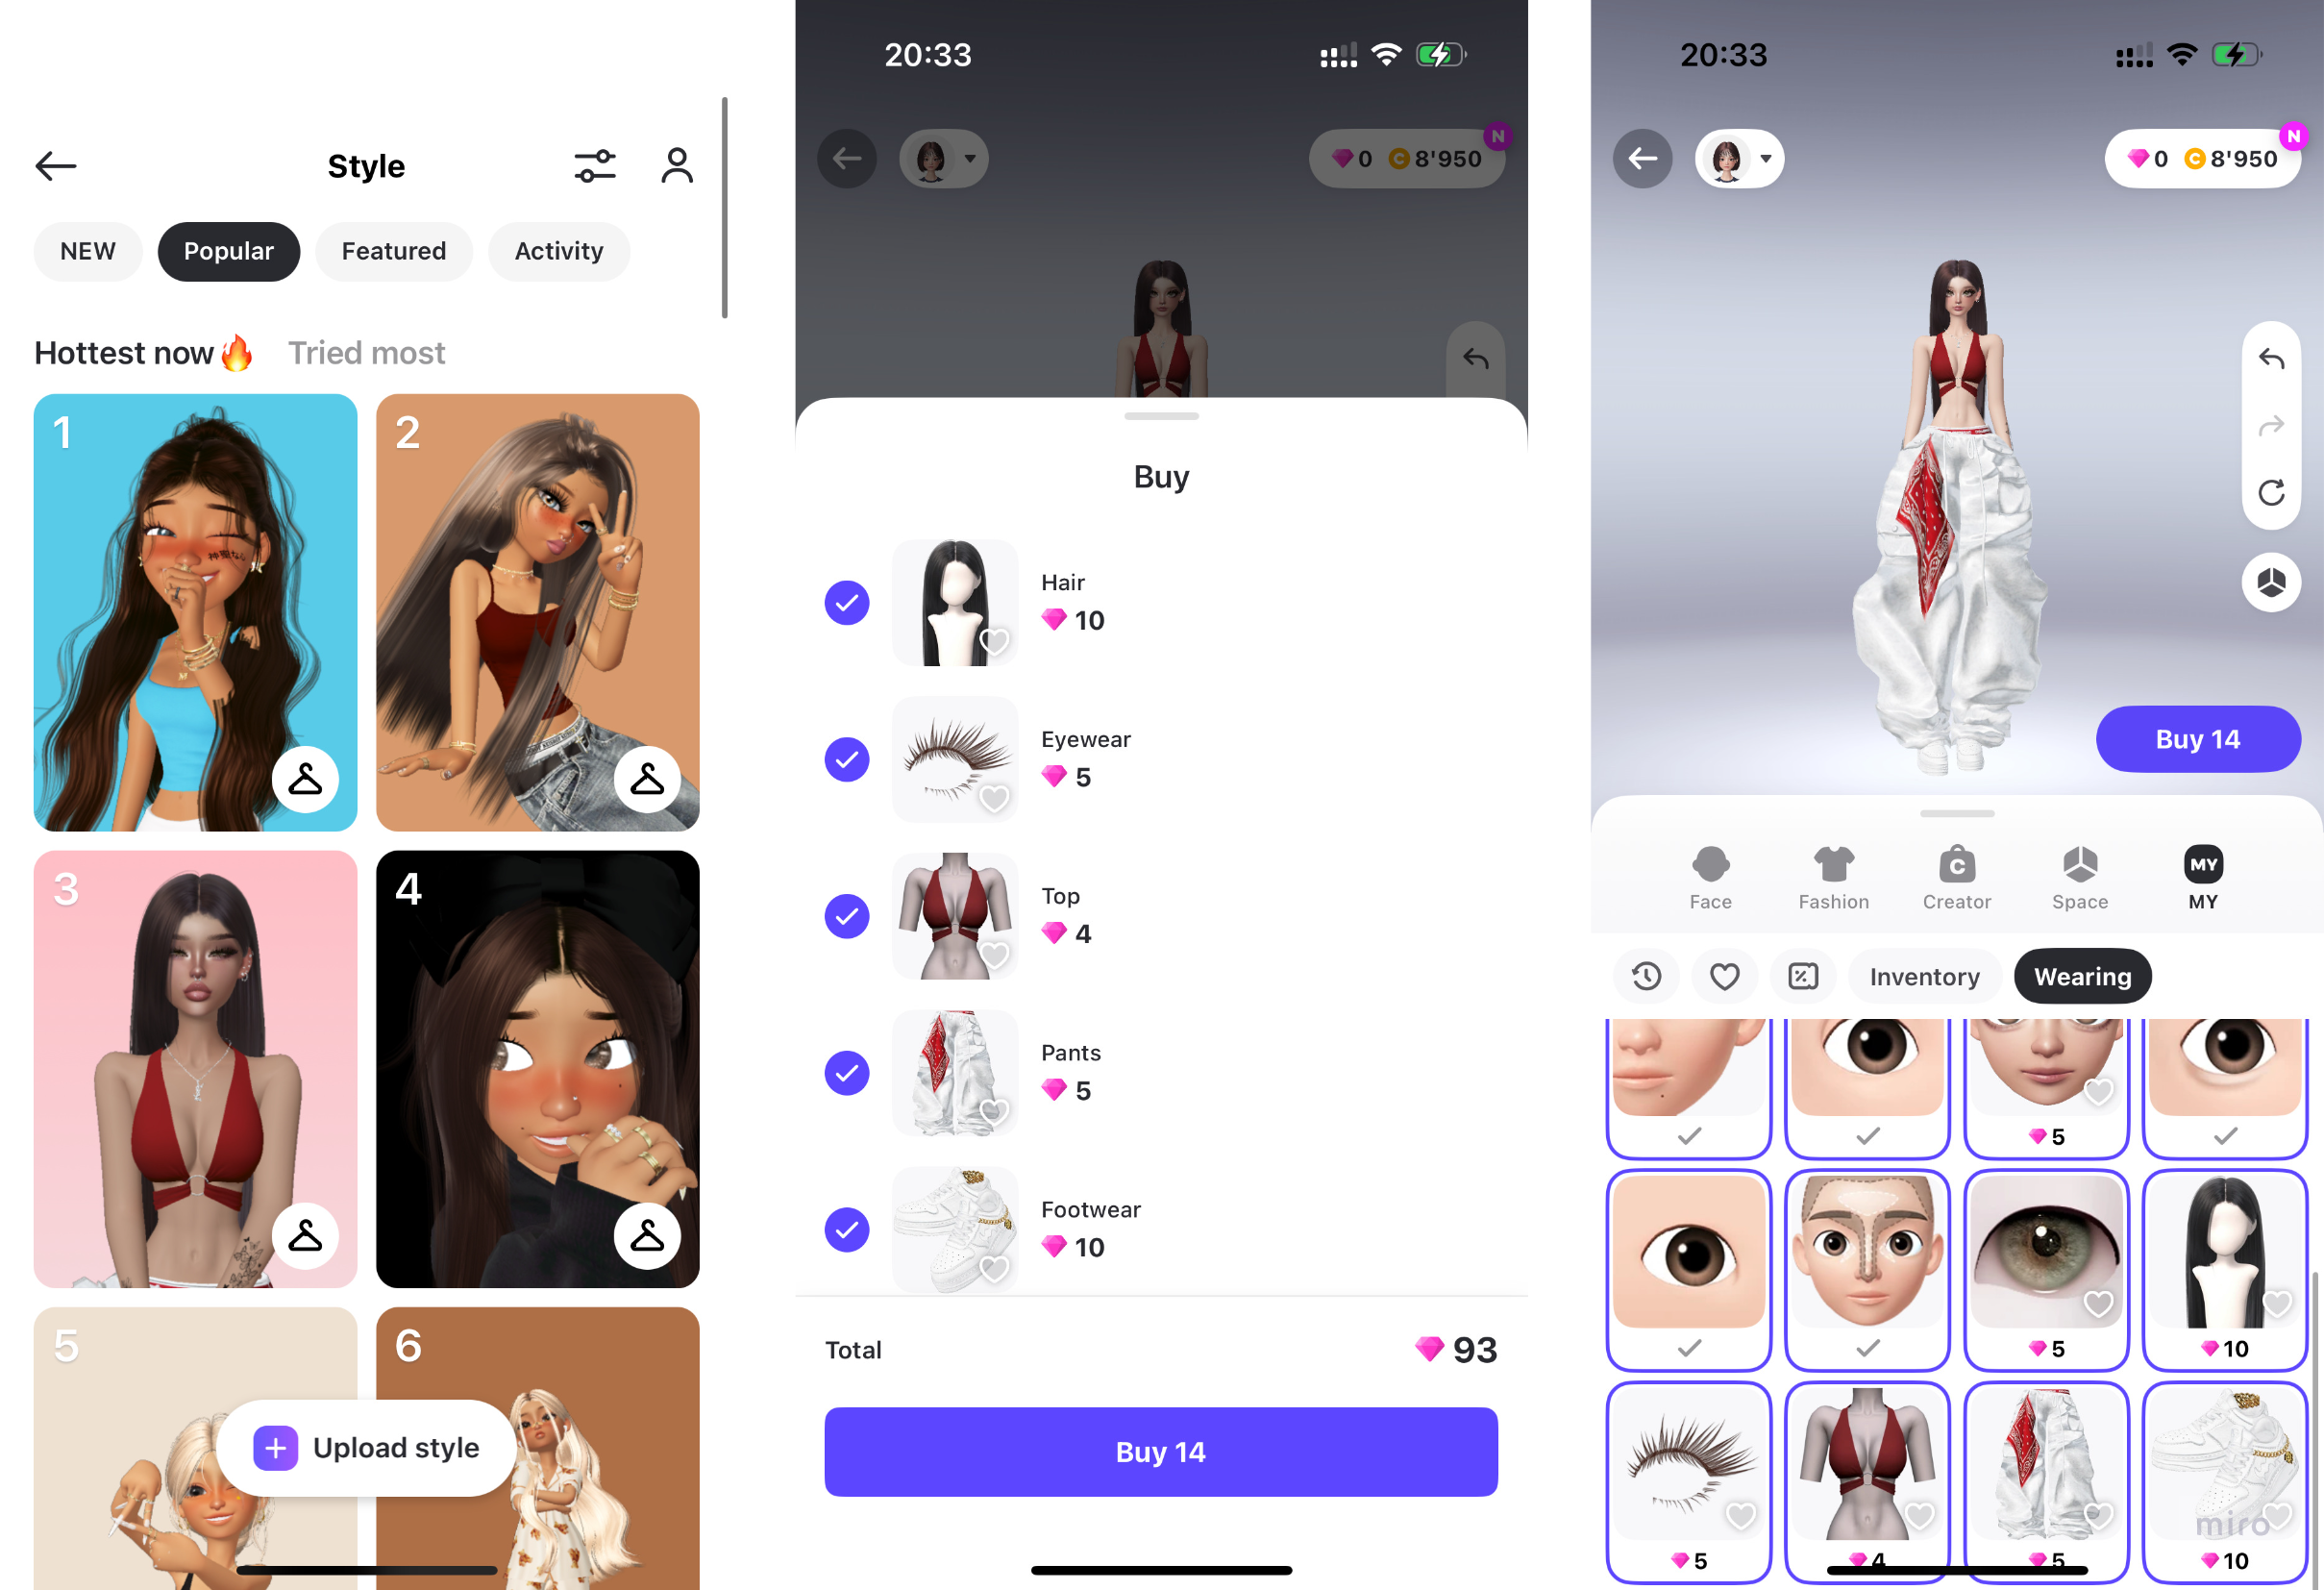
\includegraphics[width=0.7\linewidth]{template/images/chap4/zepeto_deco.png}
    \caption{Zepeto decoration}
    \label{fig:placeholder}
\end{figure}

\subsection{In-Game Elements}
\subsubsection{Customization}
Items needed to customize ZEPETO’s appearance—such as clothing, hair, and accessories—can be purchased with coins. At the start, new users are given 15,000 coins, enough to buy one or two outfits. A welcome pack (previously given as a paid ZEM item) is no longer available. Since the August 26, 2019 update, daily attendance checks allow users to earn more coins.  

ZEPETO also provides creator functions that allow users to design clothing themselves. While initially inexpensive, creator-made clothes have become more expensive. These items can be created through the ZEPETO Creator website, and their price (between 1 and 500 ZEMs) is set by the creator.  

\subsubsection{Live}
ZEPETO Live allows users to broadcast in real time using their 3D avatars. The function is built into the app, requiring no special equipment or settings. Broadcasting rights are automatically given to users with 100 or more followers. The system supports various interactive functions such as gestures, items, and backgrounds, as well as monetization through fan gifts and “boosts.”  

Different broadcasting time limits apply depending on the country. For example, Korea, Japan, France, and global regions allow 24-hour streaming, while Thailand, Indonesia, and Taiwan have time restrictions.  

\subsubsection{Gestures}
Gestures are motion items available in “Worlds.” More dynamic ones cost around 1,000 coins, while simple gestures cost 200–300 coins. Many default gestures are also provided.  

\subsubsection{Coins and ZEMs}
Coins and ZEMs are used to purchase fashion and interior items or gestures. Users often need to pay real money when they run out. ZEPETO also provides advertising and survey-based reward systems. Some of these, however, have been criticized for bugs, spam, or unfair practices.  

\subsubsection{Worlds}
Users can control their avatars to interact with others in various themed maps. Updates have added new features such as following friends.  

\begin{figure}
    \centering
    \includegraphics[width=1\linewidth]{template//images//chap4/zepeto_space.png}
    \caption{Zepeto world}
    \label{fig:placeholder}
\end{figure}

\subsubsection{Clubs}
Similar to guilds, clubs foster group-based interactions. Various crews existed earlier but were replaced in January 2024 by the new “Club” feature. However, many users still argue that clubs cannot fully replace crews.  

\subsection{Interface}
ZEPETO operates primarily on mobile and PC. Users create personalized 3D avatars using facial recognition or manual editing. Main interface features include:
\begin{itemize}
    \item Avatar customization using in-app currency.
    \item Exploration of user-generated 3D worlds (parks, cities, cafes).
    \item Social features such as chat, photo booths, and gesture interactions.
    \item An integrated marketplace for fashion and decoration items.
\end{itemize}

Unlike VRChat’s VR-based navigation, ZEPETO uses tap and joystick controls, resembling mobile RPGs or The Sims.  

\subsubsection{Visual Aesthetics}
ZEPETO emphasizes cute, trendy 3D visuals. Avatars resemble stylized dolls, matching K-pop and Korean pop-cultural aesthetics. Spaces are pastel-toned and urban, inspired by Korean cafes and studios.  

\subsubsection{Spatial Form and Navigation}
Users view avatars from a third-person perspective. Spaces range from fashion studios to theme parks, curated for events and brand collaborations. Portals enable seamless movement between spaces.  

\subsubsection{Interaction Design and Atmosphere}
ZEPETO emphasizes expressive, aesthetic-centered sociality. Main features include preset emoticons, selfies, fan events, and playful interactions. Atmosphere is light and visually driven, focusing less on deep conversation and more on curated identity.  

\clearpage

\subsection{Economic Model}
ZEPETO is based on a premium microtransaction model. Users purchase items with coins and ZEMs, while creators sell user-generated content. Partnerships with brands expand digital commerce, and premium subscription tiers (Basic and Plus) offer extra benefits.  
\begin{table}[tbph!]
	\centering{
		\begin{tabular}{ |l|c|c| }
			\hline
			& \textbf{Premium Basic} & \textbf{Premium Plus} \\
			\hline
			\textbf{ZEM Reward} & 70 ZEM per month & 170 ZEM per month \\
			\hline
			\textbf{Coin Reward} & - & 5,000 Coins per month \\
			\hline
			\textbf{Attendance Bonus} & - & 1 ZEM per day \\
			\hline
			\textbf{Premium Profile Badge} & O & O \\
			\hline
			\textbf{Creator Priority Review} & O & O \\
			\hline
			\textbf{Color Picker Use} & O & O \\
			\hline
			\textbf{Custom PRO Use} & - & O \\
			\hline
			\textbf{Premium Exclusive Items} & X (Service ends May 1, 2025) & - \\
			\hline 
		\end{tabular}
		\caption[Premium Benefits Comparison]{Comparison of Premium Basic and Premium Plus benefits in ZEPETO.}
		\label{tab:zepeto_premium}
	}
\end{table}


Coins and ZEMs are the currencies used within the ZEPETO service to purchase items.

\begin{table}[tbph!]
\centering{
\begin{tabular}{ |l|c|c|c|c|c| }
\hline
\textbf{Product} & \textbf{Original} & \textbf{Bonus} & \textbf{Android (KRW)} & \textbf{iOS (KRW)} & \textbf{USD} \\
\hline
4,680 Coin  & 4,680  & 0     & ₩1,500  & ₩1,500  & \$0.99 \\
\hline
9,700 Coin  & 9,400  & 300   & ₩3,000  & ₩3,000  & \$1.99 \\
\hline
25,200 Coin & 23,500 & 1,700 & ₩7,500  & ₩7,500  & \$4.99 \\
\hline
40,700 Coin & 37,900 & 2,800 & ₩12,000 & ₩12,000 & \$7.99 \\
\hline
110,000 Coin& 100,000& 10,000& ₩32,000 & ₩32,000 & \$20.99 \\
\hline
300,000 Coin& 272,500& 27,500& ₩87,000 & ₩87,000 & \$56.99 \\
\hline
\end{tabular}
\caption[Coin Price List]{Price list of Coins (KRW and USD).}
\label{tab:coin_price}
}
\end{table}

\begin{table}[tbph!]
\centering{
\begin{tabular}{ |l|c|c|c|c|c| }
\hline
\textbf{Product} & \textbf{Original} & \textbf{Bonus} & \textbf{Android (KRW)} & \textbf{iOS (KRW)} & \textbf{USD} \\
\hline
7 ZEM    & 7    & 0   & -        & -        & - \\
\hline
14 ZEM   & 14   & 0   & ₩1,500   & ₩1,500   & \$0.99 \\
\hline
28 ZEM   & 28   & 0   & ₩3,000   & ₩3,000   & \$1.99 \\
\hline
58 ZEM   & 56   & 2   & ₩6,000   & ₩6,000   & \$3.99 \\
\hline
128 ZEM  & 122  & 6   & ₩13,000  & ₩13,000  & \$8.49 \\
\hline
323 ZEM  & 308  & 15  & ₩33,000  & ₩33,000  & \$21.49 \\
\hline
1,000 ZEM& 934  & 66  & ₩100,000 & ₩100,000 & \$65.99 \\
\hline
2,899 ZEM& 2,706& 193 & ₩289,000 & ₩289,000 & \$190.99 \\
\hline
\end{tabular}
\caption[ZEM Price List]{Price list of ZEM (KRW and USD).}
\label{tab:zem_price}
}
\end{table}

\clearpage

\subsection{Criticism}
71\% of ZEPETO’s users are aged 7–18. This demographic often blurs the distinction between self and avatar, raising concerns about identity and safety. Although the platform enforces guidelines, risks remain.  

\section{ZEP}
% Developer Interview  
% \href{https://blog.naver.com/zep_business/223381916310}  

% \textbf{Is there a special reason why your developer community uses ZEP?}  
% Being able to code individually in the same space while visiting community members whenever needed seemed to fit well with the purpose of “Mogakco” (gathering together to code separately).  

% Even though we were coding in different physical spaces, simply being together in the same virtual space gave us a sense of belonging. With occasional small talk and development-related discussions, we were able to create a more focused environment.  

% \textbf{Have you tried doing Mogakco through other platforms?  
% If so, why do you specifically use ZEP instead of those platforms?}  

% A. I really liked being able to measure absolute study time through the study app. Of course, I could use other applications, but with ZEP I didn’t need to leave the space to use other apps—it was convenient to proceed directly within the same space. Also, ZEP’s character sprites are cute. Compared to other platforms, they are cuter and more appealing, which made communication inside the space more enjoyable. I also often purchase paid items such as effects or the “poke” function because they look nice.  

% Previously, I tried Mogakco through Discord, but since it is in messenger format, it only shows login status with a green light. It didn’t give me the feeling of actually studying together, which was disappointing. On ZEP, however, the space itself gave me the sense of studying together even when physically apart, and it provided interaction tools like “poking.” Since there are also cute characters, it felt possible to express direct reactions—for example, if someone made a bad joke, the avatar could turn away with a blank expression.  

% A. Having people represented as characters in the same space! I think the other features are additional functions that maximize the sense of being together in one space. Even though we are physically far apart, the feeling of being in the same space was the best part. I believe that if you use the app well, you can maximize that advantage.  



ZEP is a Korean metaverse platform developed by Naver Z, a subsidiary of Naver Corp. and the company behind the virtual avatar platform ZEPETO. Launched in 2022, ZEP (short for “Zeppelin”) was created in collaboration with Naver Cloud. It focuses on improving productivity, community events, and education within virtual environments. Unlike its sibling platform ZEPETO—which targets Gen Z’s social expression and avatar customization—ZEP is designed for practical group use cases such as remote team meetings, online classes, and hybrid community events.  

ZEP has quickly gained popularity in Korea, especially among young professionals, students, and public institutions seeking a more engaging alternative to Zoom. After its official launch, it recorded 1 million cumulative users within six months, and surpassed 7.7 million users one year later.  

\begin{figure}
    \centering
    \includegraphics[width=1\linewidth]{template//images//chap4/zep.png}
    \caption{zep}
    \label{fig:placeholder}
\end{figure}

\subsection{In-Game Features}
Although ZEP is a browser-based metaverse platform, it does not remain only a space for meetings or education. It actively incorporates game-like elements designed to allow users to experience fun and belonging. These core elements include customization, mini-games, and quiz/participatory functions.  

\subsubsection{Customization}
\begin{itemize}
    \item Avatar customization: express individuality through hairstyles, clothing, and accessories.  
    \item Space customization: decorate personal rooms or self-created maps.  
    \item Creator tools: with drag-and-drop tools, anyone can create maps or items → expands users from consumers into creators.  
    \item Community sharing: customized avatars or spaces can be shared with other users or used in events → identity expression + communal belonging.  
\end{itemize}

\subsubsection{Mini-Games}
\begin{itemize}
    \item Built-in content: light, accessible games such as jump maps, mazes, races, tag, and quests.  
    \item Social play: cooperation or competition possible through friend invites or random matching.  
    \item Interactivity: chat, emotes, and item use during play → relationships form naturally through play.  
    \item UGC-based: anyone can design mini-games using ZEP’s map-making tools → games become user-generated content.  
    \item Extended play: activities lead to secondary cultures such as sharing screenshots, fashion displays, or parties.  
\end{itemize}

\subsubsection{Quiz}
\begin{itemize}
    \item Live QA app: hosts ask questions, participants respond in real time → supports quizzes, surveys, and polls.  
    \item Reward/feedback system: provides instant feedback and rewards → increases immersion.  
    \item Fandom usage: used in idol events or fan meetings to strengthen fan-artist belonging.  
    \item Extended elements: roulette, gifts, reaction emotes can be embedded into maps → turns audiences into participants rather than mere spectators.  
\end{itemize}

\subsection{Interface}
ZEP’s interface is similar to Gather.town, offering a top-down 2D pixel-art environment with RPG-like avatars. Users move through customizable spaces using arrow keys and interact with objects (desks, screens, doors) containing video, documents, or portals.  

Main features include:
\begin{itemize}
    \item Spatial video chat (audio activated when avatars are close).  
    \item Built-in productivity tools (e.g., Miro board, PDFs, timers).  
    \item Editable maps and drag-and-drop customization.  
    \item Administrative tools for hosting events, role assignment, and attendance tracking.  
\end{itemize}

ZEP’s Korea-focused design includes native integration with NAVER services. Its UI is often optimized for Korean language and cultural conventions (e.g., digital name tags, polite language filters).  

\subsubsection{Visual Aesthetics}
ZEP (provided by Naver Z) uses a top-down 2D pixel style similar to Gather but with distinct differences in visual aesthetics, atmosphere, and cultural references. Compared to Gather, ZEP’s style feels more modern and refined. Despite being pixel art, it uses more detailed designs and subtle gradients to create clean and smooth images.  

Avatars are cuter and more expressive, offering a warm and expansive visual perspective. This style connects to Korean character aesthetics such as Kakao Friends and LINE Friends.  

ZEP’s virtual spaces are richly decorated, often resembling stylish classrooms, cafes, and cozy coworking offices. These designs seem inspired by popular offline coworking spaces in Korea, providing familiar and comfortable emotional cues. Overall, ZEP’s environments are designed to promote both social interaction and digital productivity, with a warm and welcoming atmosphere.  

\begin{figure}
    \centering
    \includegraphics[width=1\linewidth]{template//images//chap4/zep_space.png}
    \caption{zep space}
    \label{fig:placeholder}
\end{figure}

\subsubsection{Spatial Form and Navigation}
Like Gather, ZEP uses a top-down, avatar-based navigation system, with movement controlled via arrow keys or WASD. However, ZEP’s spatial composition reveals a clearer orientation toward organized, task-based structures.  

Key features and spatial structures:
\begin{itemize}
    \item Pre-designed templates: default spaces include classrooms, team-building rooms, and open collaboration areas designed for practical communication and collaboration.  
    \item Interactive boards and shared document functions: strong integration with productivity tools such as Google Docs and whiteboards, suitable for workshops or educational contexts.  
    \item Object interactions: in-world objects include games, YouTube screens, PDFs, timers, etc., enabling diverse content consumption without leaving the platform.  
\end{itemize}

\subsubsection{Interaction Design and Atmosphere}
ZEP is optimized for collaborative work, education, and fandom-based gatherings. Unlike Gather’s looser, more game-like sociality, ZEP offers structured spaces for soft but cohesive collaboration.  

The platform supports both:  
\begin{itemize}
    \item Formal meetings (e.g., classroom-style environments using host tools).  
    \item Informal gatherings (e.g., ZEP-based virtual fan meetings or study rooms).  
\end{itemize}

Interaction layer elements include:
\begin{itemize}
    \item Proximity-based voice (optional).  
    \item Pop-up chat boxes designed for high visibility in public spaces.  
    \item Integrated media tools (YouTube player, timers, schedules).  
    \item Emoji reactions and name tags that allow soft emotional signaling without violating norms.  
\end{itemize}

\cleardoublepage

Cultural context and spatial design:  
ZEP reflects the Korean digital trend of “Mogakgong” (gathering together to study separately) while also supporting structured activities such as countdowns, polling boards, and quizzes. This duality illustrates how Korean digital culture fuses personal expression with collectivist behavior.  

\begin{figure}
    \centering
    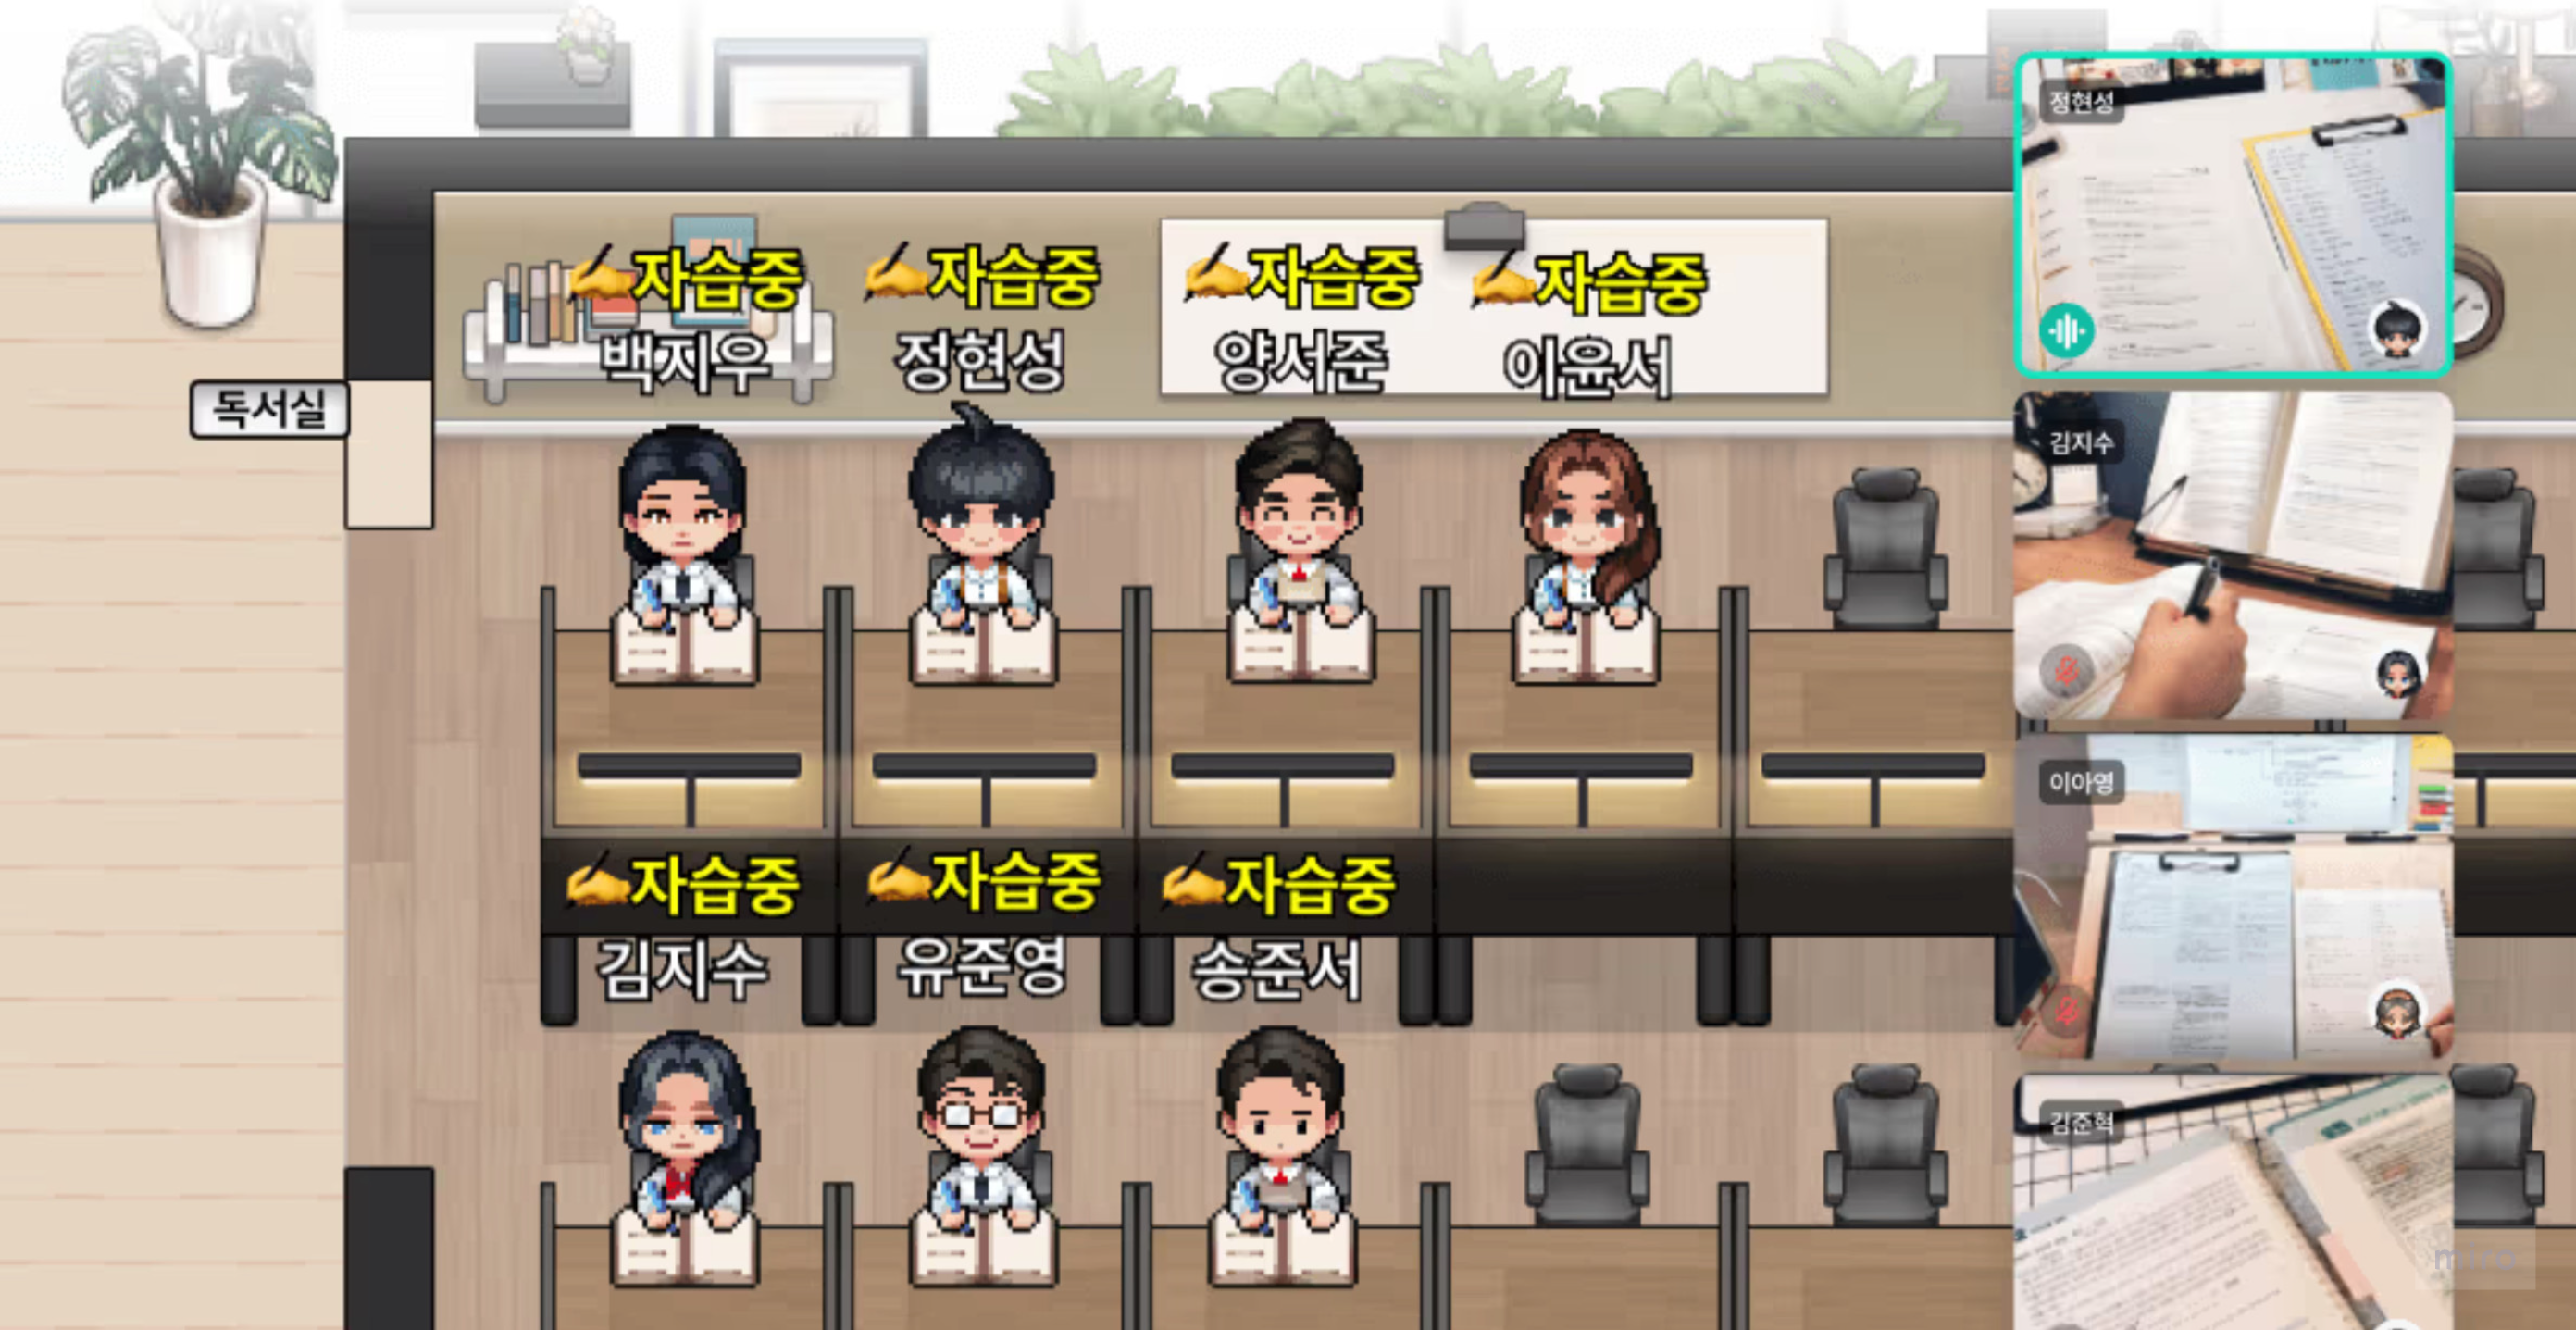
\includegraphics[width=1\linewidth]{template//images//chap4/zep_study.png}
    \caption{zep study gathering}
    \label{fig:placeholder}
\end{figure}

\cleardoublepage

\subsection{Economic Model}
ZEP offers four plans—Free, Basic, Pro, and Enterprise—with differences in available features. Unlike ZEPETO, it does not (yet) include an in-app economy or avatar marketplace, focusing instead on practicality rather than entertainment.  

\begin{figure}
    \centering
    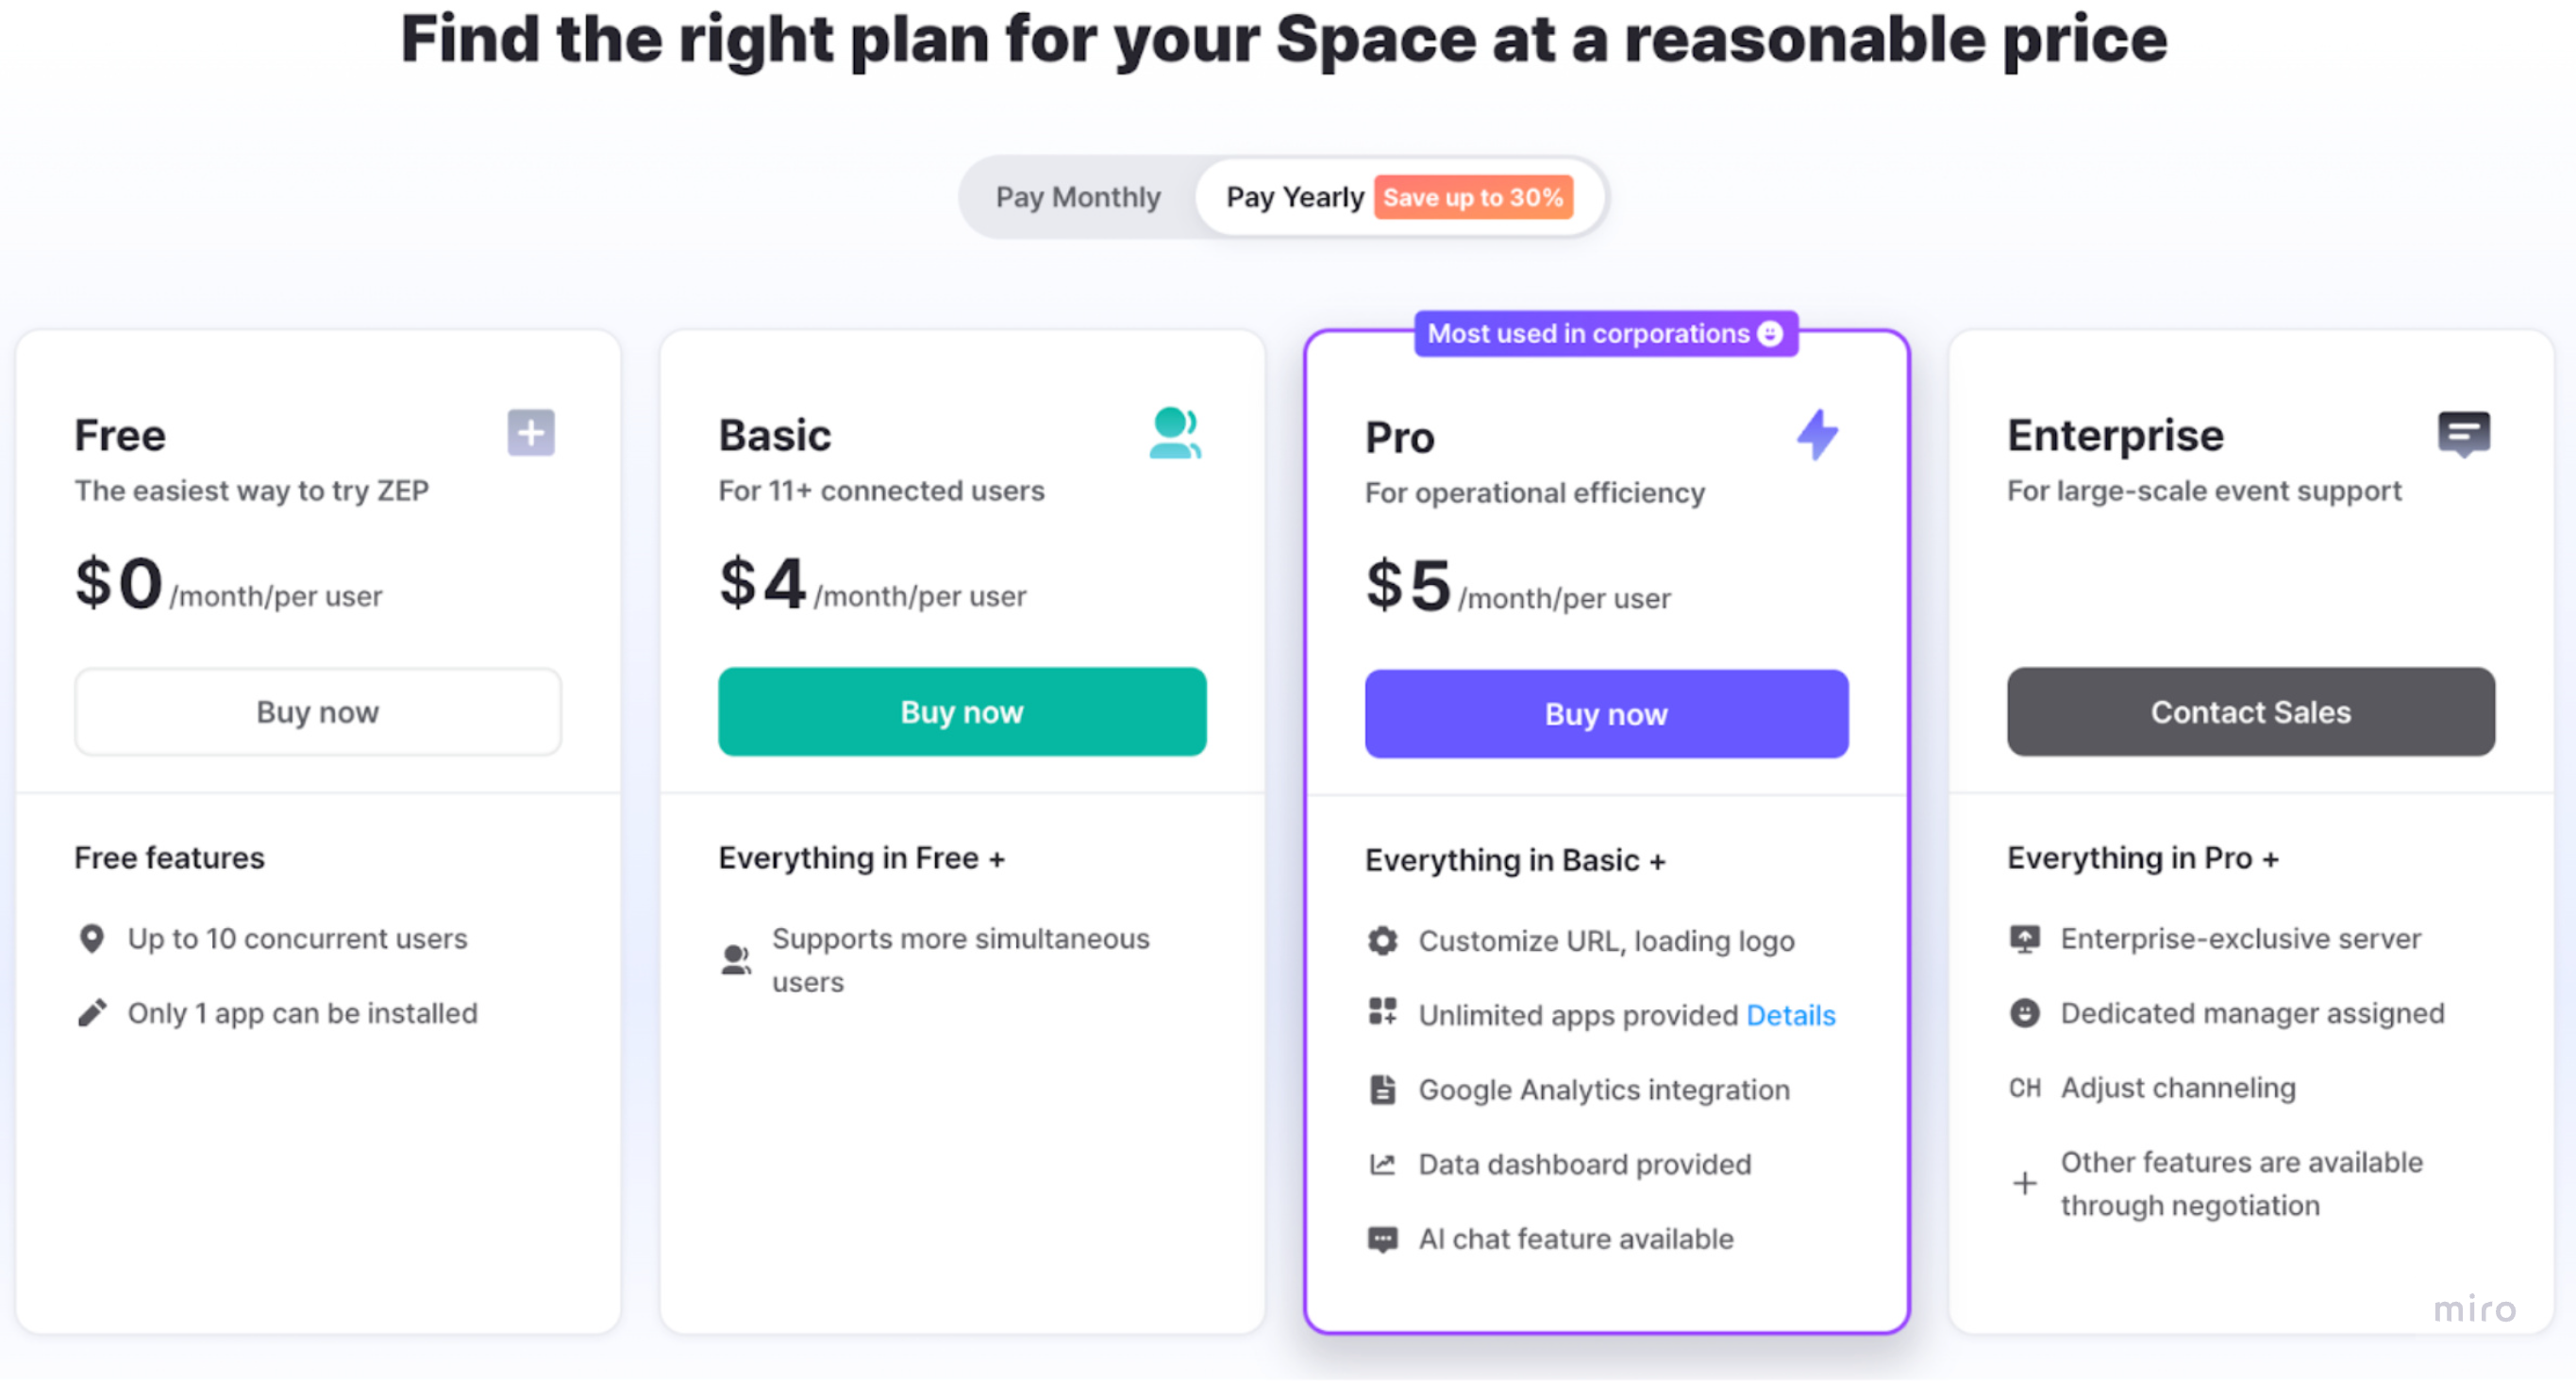
\includegraphics[width=1\linewidth]{template//images//chap4/zep_pricing.png}
    \caption{zep pricing plan}
    \label{fig:placeholder}
\end{figure}

\cleardoublepage

\section{VTubers (Virtual YouTubers)}
A VTuber is an online broadcaster who uses a virtual avatar that mimics their facial expressions and movements via camera or motion capture technology. The term was first established by the Japanese YouTuber Kizuna AI, considered a pioneer of the field.  

\begin{figure}
    \centering
    \includegraphics[width=1\linewidth]{template//images//chap4/vtuber.png}
    \caption{Vtuber}
    \label{fig:placeholder}
\end{figure}

Recently, the VTuber phenomenon has grown rapidly, showing how digital identity play in a post-family society can evolve into emotional belonging and community. While based on a real person’s voice and actions, what fans interact with is the avatar. This allows playful, fluid identities to be performed online.  

Fans do not remain passive consumers: they participate via live chat, memberships, super chats, and fan art, collectively building the VTuber’s identity and world. Through this, they experience emotional intimacy and solidarity that traditional families cannot provide. This illustrates how personal data and emotions come together to form “living networks.” In Korea, where single-person households and family decline are accelerating, VTuber fandom shows that people still long for belonging, with digital fandoms functioning as alternative family-like communities.  



\section{Twitter Role-Playing}
Role-playing (RP) online refers to adopting a character and performing dialogues and actions as if in character.  

\subsection{Twitter Bots}
Twitter bots are accounts linked to X’s API that post automatically, as well as accounts run manually for role-playing purposes (RPAs). While “bot” originally implied automation, in Korea it has expanded to include character role-play accounts. Bots may be official (authorized by creators) but are usually fan-created, often as a form of secondary creation.  

\subsection{Character Bots}
Character bots perform fictional personas, usually from anime, manga, or games. They allow fans to engage with favorite characters and experience the feeling of “becoming loved” through proxy interaction.  

Competition often arises to “claim” new characters by creating bots as soon as updates are announced, even before official information is released.  

\subsection{Related Research}
Yoon Myunghee and Son Subin (2015) analyzed Twitter bots as cases of identity play, showing that digital interaction is not just automated but co-constructed between managers and followers. Through role-play, fans co-create shared “worldviews” and generate playful intimacy, forming new social bonds not based on kinship but on imagination.  

This resonates with the thesis’s concept of the living network: in post-family Korean society, emotional and digital traces evolve into communal organisms. Digital spaces, thus, are not merely platforms but experimental grounds for alternative family-like relations.



% \section{Discord}
% 사실상 현재는 게이밍 메신저의 대명사로, 채팅, 통화, 화면 공유 등을 지원하는 인스턴트 메신저. 2015년 5월 13일에 모바일 MOBA 게임이었던 Fates Forever를 지원하기 위하여 출시되었다.

% 주로 온라인 게임을 즐기는 게이머들이 많이 이용하는 메신저 프로그램, 뛰어난 성능과 간편함을 바탕으로 게이머들이 과거 애용하던 주류 메신저들을 뛰어넘고 현재 주요한 앱으로서 자리하게 되었다. 디스코드의 서버 위치는 보이스 채팅에만 해당된다. 텍스트 채팅 트래픽은 전부 미국 동부의 데이터 센터에서 처리된다.

% YouWeb's 9+ Incubator라는 창업 지원 센터를 통해 초기 지원과 자금을 확보하고 Benchmark Capital과 텐센트가 투자하며 개발된 Electron 기반 프로그램이다. 개발자들은 Skype, Slack, TeamSpeak와 같은 VoIP 소프트웨어의 장점들만을 모아서 낮은 대기 시간을 가진 VoIP 소프트웨어를 개발하고자 하였고, 각종 e스포츠 및 LAN 토너먼트 게이머들에게서 대중화되었다. 덕분에 2022년 상반기 기준, 전 세계적으로 3억 9,000만 명 이상의 사용자를 가지고 있다고 발표했으며, 한 달에 적어도 한 번 접속하는 유저가 약 1.5억 명이다. 현재는 트위치 등의 스트리머들을 통해 많이 알려져 있고 한국에서도 스트리머를 비롯한 인터넷 방송인을 포함하여 여러 게임 커뮤니티에서 주로 사용하고 있는 메신저이다. Discord Inc.라는 이름의 회사는 OpenFeint라는 다른 모바일 메신저를 운영하던 Jason Citron이 설립했으며 OpenFeint와는 별개로 독립적인 회사로 운영해 나간다고 발표한 적 있다. OpenFeint는 2016년 1월에 2,000만 달러를 투자하였다. 초창기에는 단순히 음성 채팅과 일반 채팅 기능만 지원하는 업무용 메신저인 슬랙의 짝퉁 수준이었다. 하지만, 슬랙은 기본적으로 기업용이다 보니 대부분의 기능이 유료인 데다, 업무 생산성 향상에 특화된 기능 위주[9]로 발전한 것에 비해, 디스코드는 게이머와 일반 사용자를 타깃으로, 간편하고 빠른 음성 채팅, 오버레이를 위시한 직관적이고 게임 친화적인 기능 등의 다양한 업데이트를 통해 차별화를 이루어 냈다.

% 또한 채팅 및 음악 봇 등 봇을 만들 수 있는 API도 지원하여 서버를 관리하거나 음악을 틀어주는 등 편리한 기능들을 제공하고 있다. 초창기부터 유저 커뮤니티를 활성화시키면서 피드백을 적극적으로 수용한 점도 성공 요인으로 뽑힌다. 파편화되어 있던 게임 커뮤니티를 디스코드로 끌어모은 것이다.

% \begin{figure}[tbph!]
% 	\centering
% 	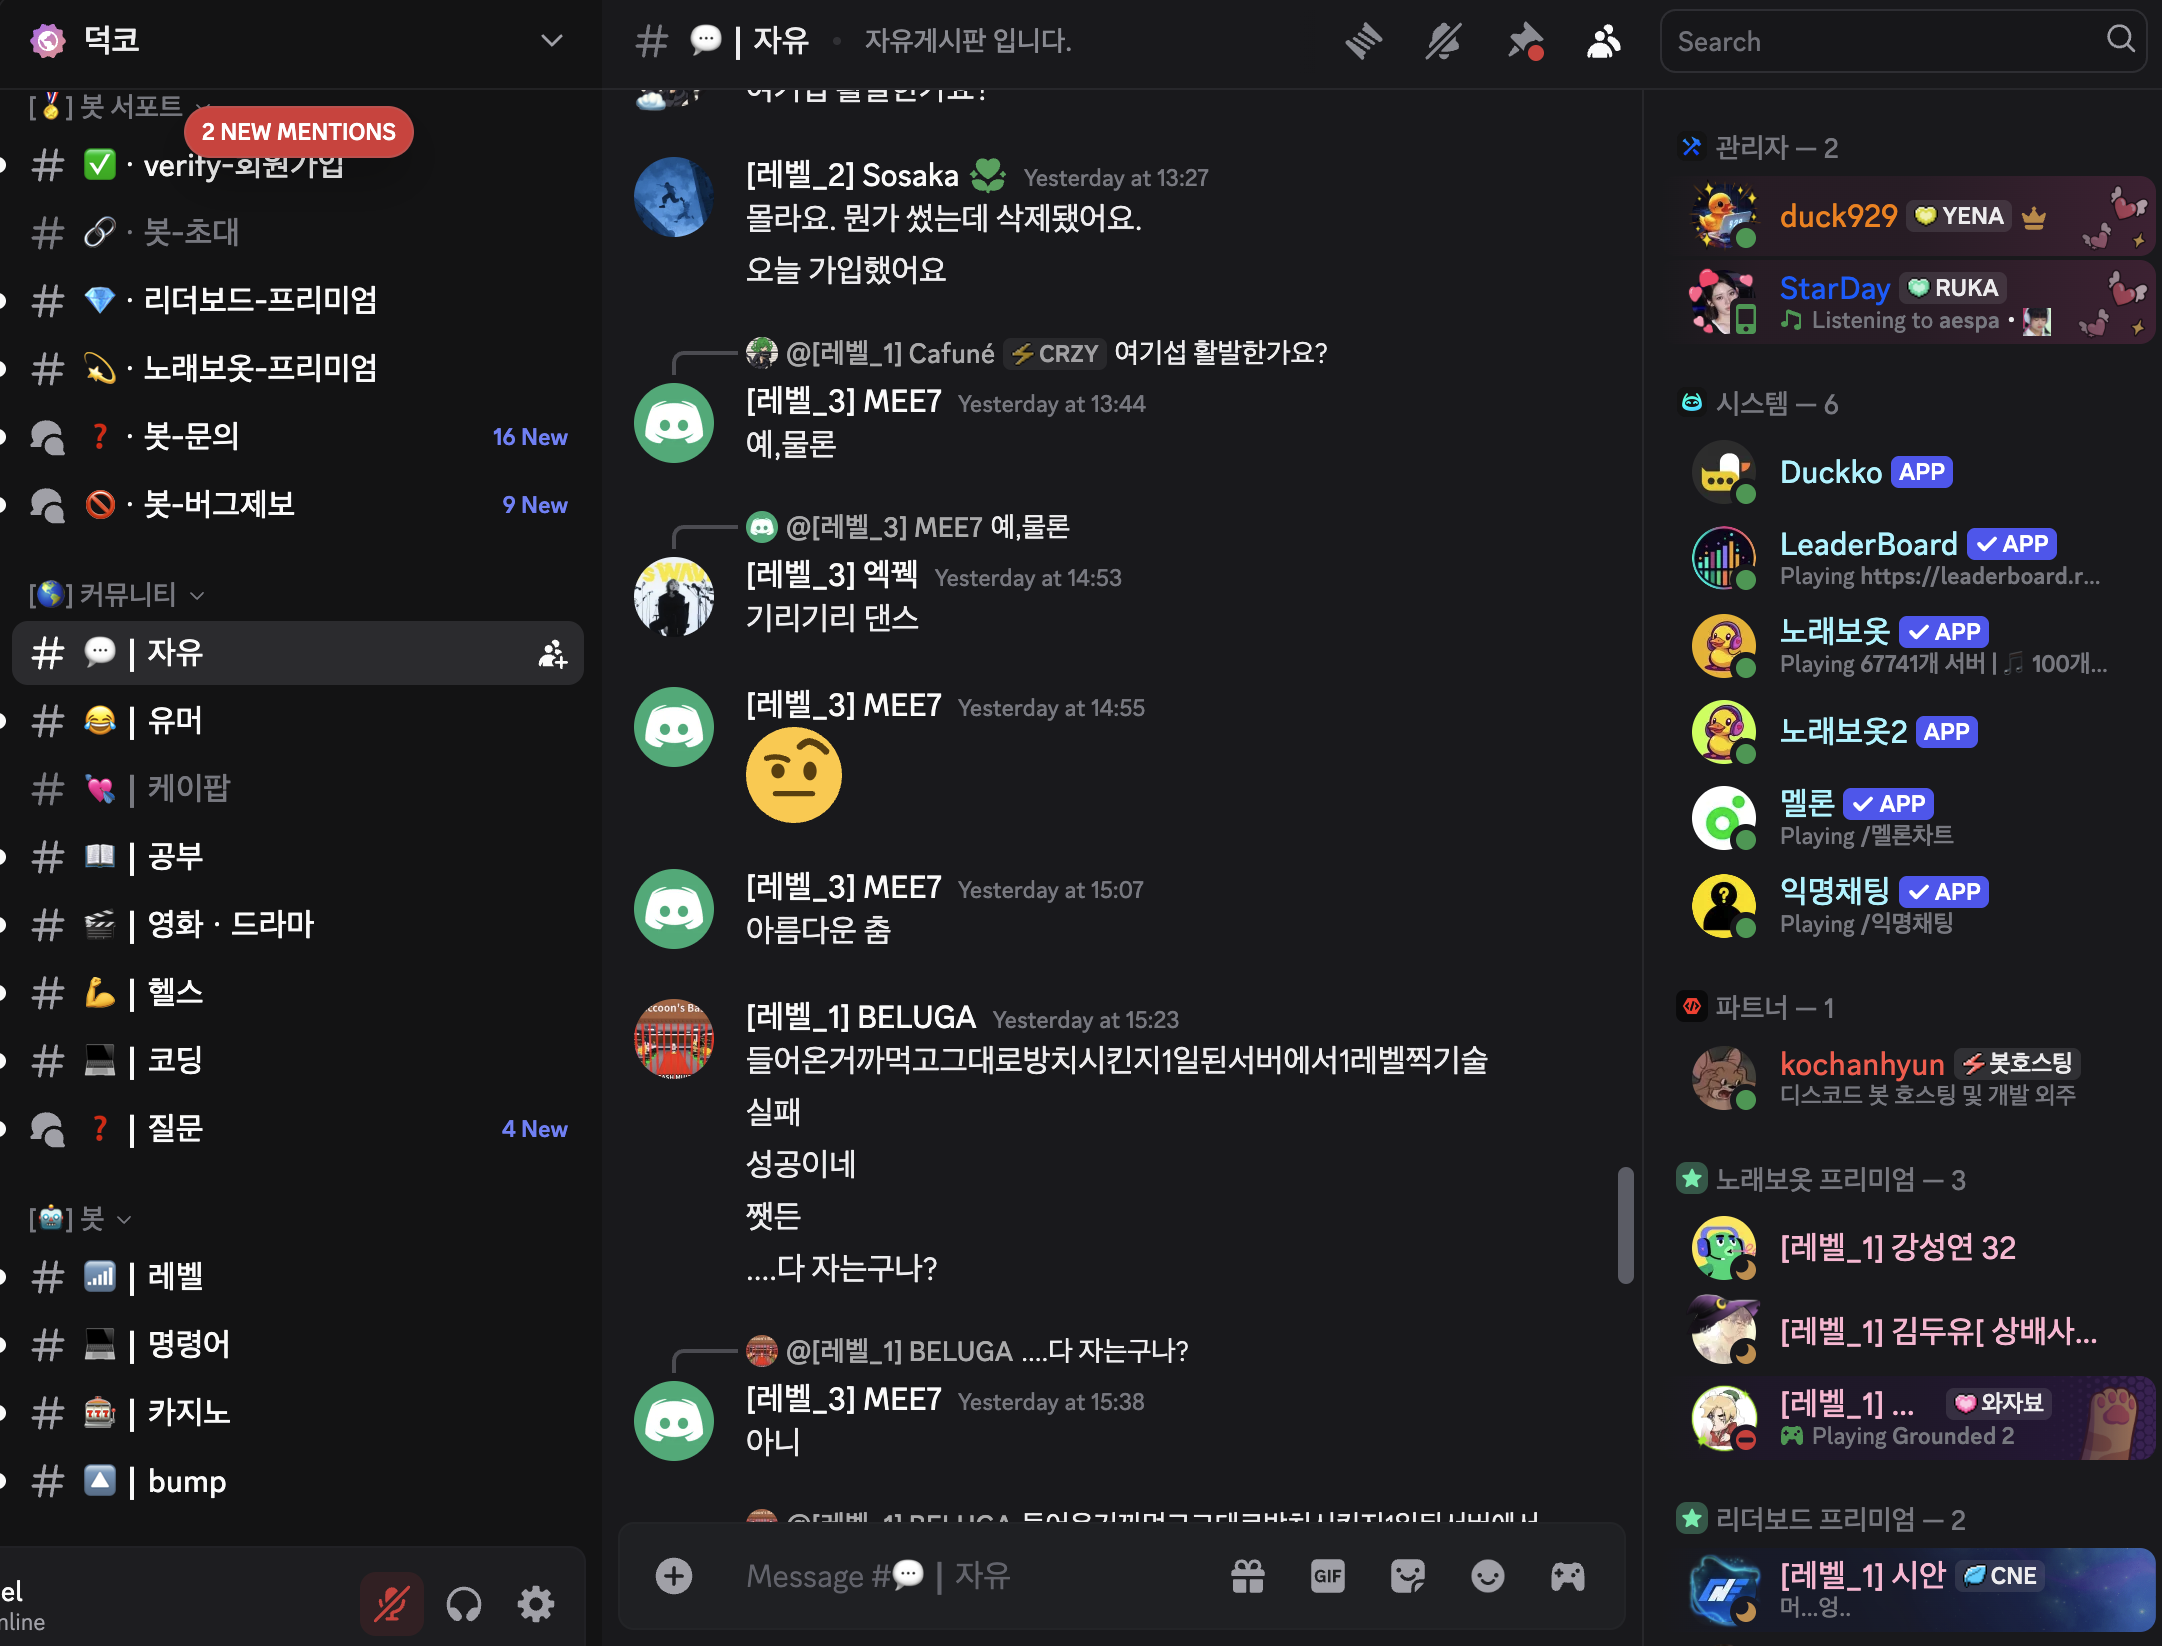
\includegraphics[width=0.7\linewidth]{template/images/chap4/discord.png}
% 	\caption[Discord]{Discord}
% 	\label{fig:image}
% \end{figure}

% \section{Kakaotalk Open chat}
% 오픈채팅방 또는 오픈카톡방은 카카오톡에서 오픈채팅을 위해 만들어진 오픈채팅 커뮤니티를 뜻한다.

% 오픈채팅방은 오픈 채팅을 통해 취미, 친목을 진행하거나 정보교환, 공부를 목적으로 개설된다. 가족 혹은 친구들이 연락을 위해 형성하기도 하며, 직장에선 업무 지시를 위해 오픈채팅방을 개설하기도 한다. 개중에선 정보를 유료로 판매하는 유료 공유방, 유료 단톡방같은 형태도 존재한다.

% 단톡방(그룹채팅)과 흔히 혼용되곤 하는데, 단톡방은 카카오톡에서 등록된 친구를 초대하여 만들어지는 형식이며, 오픈채팅방은 채팅방 링크를 통해 접속이 가능하다는 차이가 있다. 다만 다른점은 오픈채팅방은 단톡방과 달리 소셜 네트워크 상에서 검색이 가능하며, 방장의 권한하에 가입할 때에 비밀번호를 요구하기도 한다. 또한 오픈채팅은 단톡방에 없는 방장과 최대 10명까지의 부방장을 두는 관리자 시스템이 존재하고 그로 인해 채팅방 내의 인원에게 방장 변경이 가능하며[1] 또는 내보내기가 가능해진다.[2]
% 한마디로 단톡방은 지인들의 모임이라고 볼 수 있고, 오픈채팅방은 완전히 공개된 광장이라고 볼 수 있다. 말 그대로 오픈 채팅이다.

% 오픈 채팅방은 메신저형 소셜 네트워크와 장점을 공유한다. 여러 사람이 동시에 소통할 수 있으며, 실시간으로 참여하지 않더라도 남겨진 메세지를 통해 수월하게 소통할 수 있다. 또한 접속만 하고 있다면, 참여 여부와 상관없이 인원과 채팅내역이 지속된다.

% 파일, 목소리, 단체통화 등 여러 형태로 소통이 가능하며 연동된 앱에 따라선 송금, 선물하기 등의 행위까지 수월하게 할 수 있으며, 대부분 모바일이 연동되므로 비교적 접속과 참여가 자유롭다.

% \begin{figure}[tbph!]
% 	\centering
% 	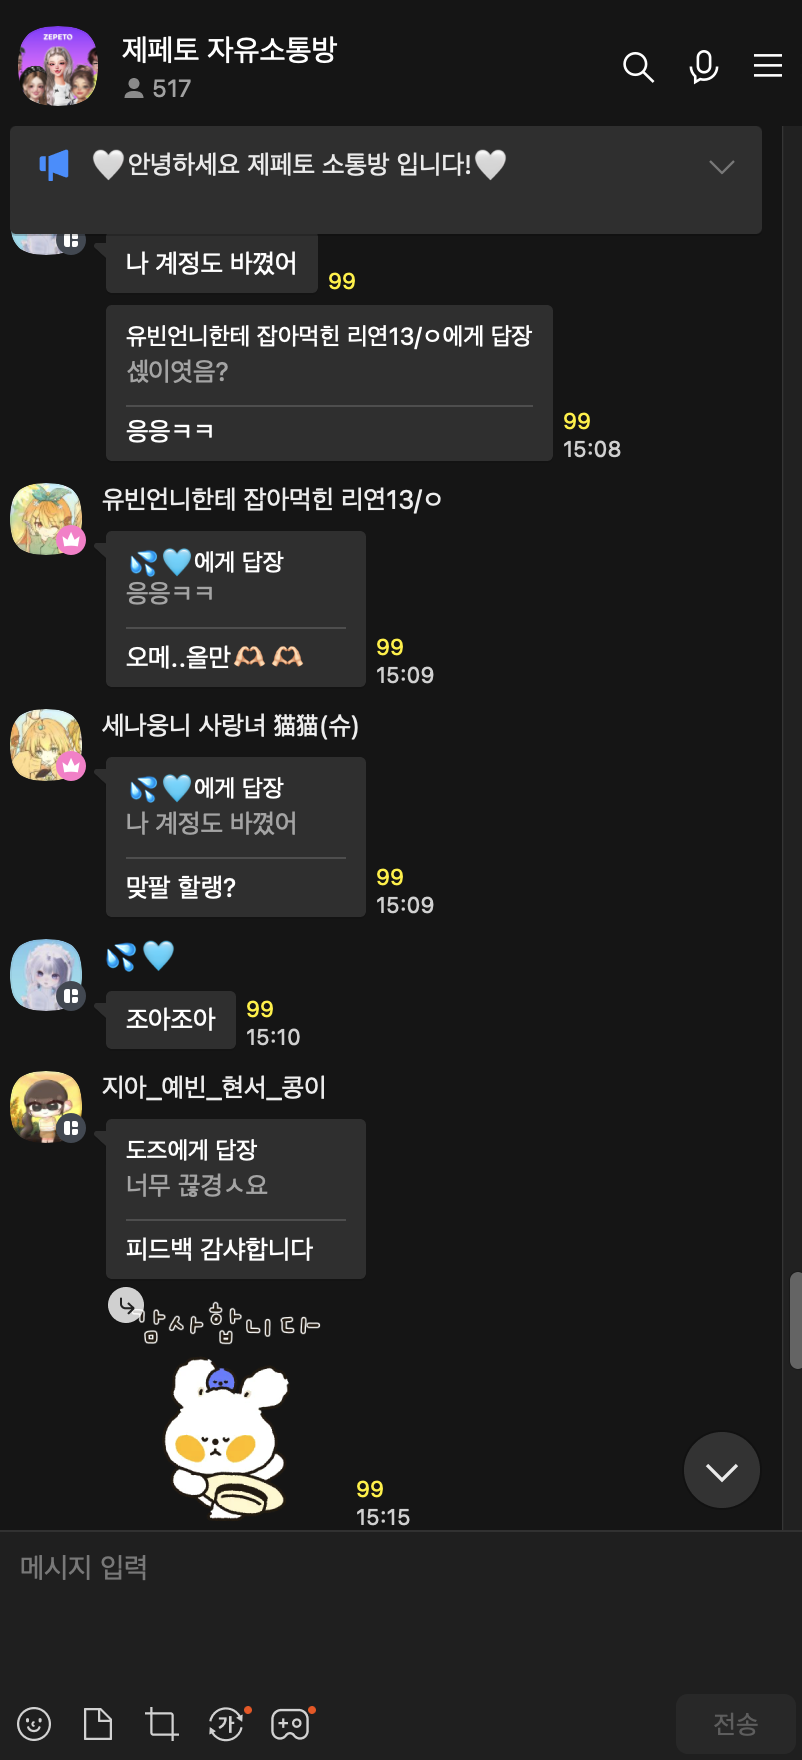
\includegraphics[width=0.3\linewidth]{template/images/chap4/kakaotalk.png}
% 	\caption[Kakaotalk]{Kakaotalk}
% 	\label{fig:image}
% \end{figure}

% \section{ZEPETO, Enjoy?}
% 네이버제트가 운영하는 증강현실 (AR) 아바타 서비스로, 대한민국 대표적인 메타버스 플랫폼이다. 2018년 출시된 제페토는 얼굴인식과 증강현실 (AR), 3D 기술 등을 이용해 ‘3D 아바타’를 만들어 다른 이용자들과 소통하거나 다양한 가상현실 경험을 할 수 있는 서비스를 제공한다. 제페토는 인공지능(AI) 기반의 얼굴인식 기술을 통해 '또 다른 나'인 3D AR 아바타를 만들어 가상공간에서 지인, 친구와 소통할 수 있는 새로운 형태의 SNS(사회관계망서비스)다. 출시 두 달 만에 글로벌 앱 다운로드 수가 300만 건을 넘어섰고, 약 2년 만에 누적 가입자 수가 3억 4000만 명을 돌파했다. 이 중 해외 이용자 비율이 90% 이상이다.

% 산리오 캐릭터즈와 스누피 등의 유명 브랜드와의 제휴도 활발하며, 제페토에 다양한 콘텐츠를 제공하므로써 인기를 끈다. 구찌, 나이키, 휠라 등 패션업계도 제페토와 협업해 패션아이템 등 디지털 굿즈를 만들어 판매하기도 했다.

% 분사 후 제페토는 자체적인 아바타 플랫폼 생태계 구축과 글로벌 확장에 집중한다. 제페토는 향후 이용자들이 의상을 비롯한 다양한 아이템을 직접 제작하고, 또 판매까지 할 수 있는 제페토만의 창작자 플랫폼 '제페토월드'를 구축하였다. 모바일과 pc에서 모두 사용 가능하다. 

% \begin{figure}
%     \centering
%     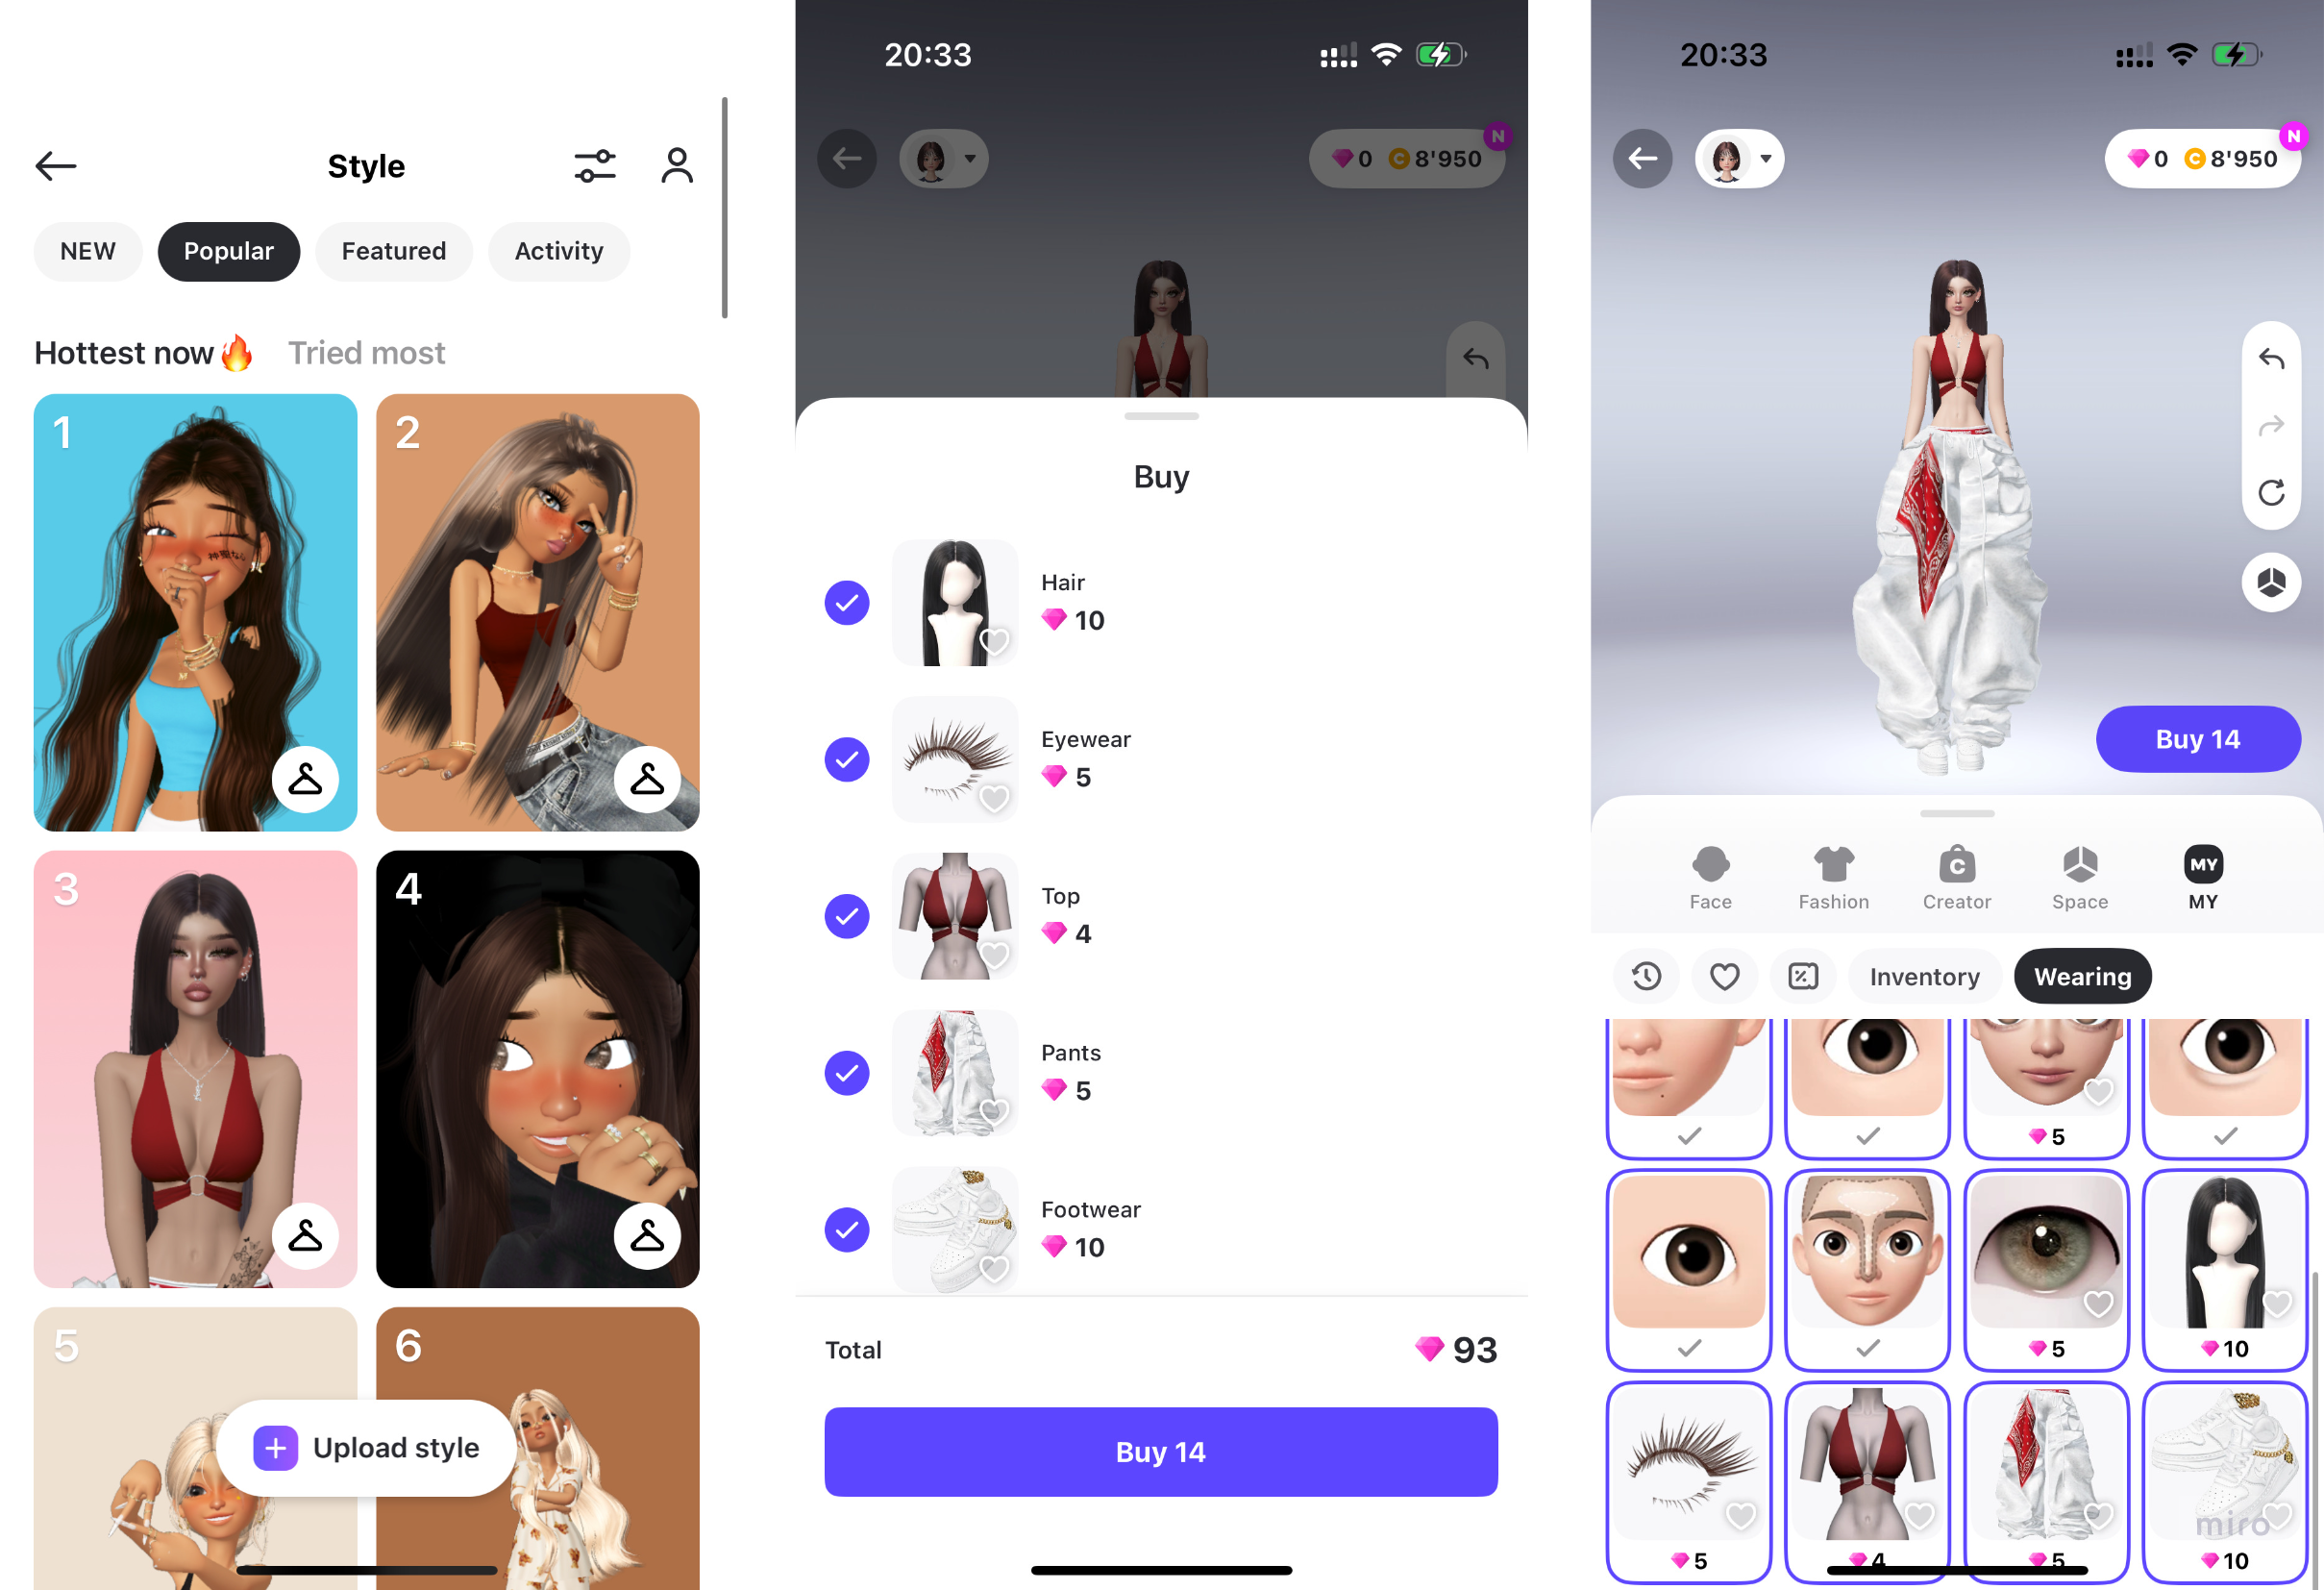
\includegraphics[width=0.7\linewidth]{template/images/chap4/zepeto_deco.png}
%     \caption{Zepeto decoration}
%     \label{fig:placeholder}
% \end{figure}


% \subsection{게임 내 요소}
% \subsubsection{꾸미기}
% 제페토의 외형을 꾸미기 위해 필요한 아이템들로, 코인을 사용하여 의상이나 헤어, 액세서리 등을 구입할 수 있다. 웬만한 의상 한두 벌쯤은 제페토를 처음 시작할 때 지급되는 15000코인으로 구매가 가능하다. 또한 새로 시작하는 뉴비에게는 웰컴팩 (젬으로 구매할 수 있는)을 주었지만 현재는 주지 않는다.[5] 2019년 8월 26일 업데이트 기준으로 출석체크 기능이 생겨 더 많은 코인을 획득할 수 있다.

% 직접 옷을 제작할 수 있는 크리에이터 기능도 있다. 가격이 대부분 저렴한 편인데, 모든 옷을 젬으로만 구매할 수 있다. 초반과는 달리 크리에이터 옷 역시 가격이 올라가고 있다. 크리에이터 아이템은 제페토 크리에이터 웹사이트를 통해 만들 수 있으며, 가격도 그 아이템의 크리에이터가 정할 수 있다. 가격은 1젬 이상 500젬 이하여야 한다.

% 스타일은 현재 자신의 코디를 올리고 좋아요(박수)를 받는 곳이다. 그리고 해당 스타일 그대로 구매도 가능하다. 자신과 같은 상의를 입고 있는 사람들도 볼 수 있다. 좋아요는 여러 번 누를 수 있다.

% \subsubsection{라이브}

% 제페토 라이브는 사용자가 자신의 3D 아바타를 이용해 실시간 방송을 진행할 수 있는 기능이다. 방송은 제페토 앱 내에서 이루어지며, 별도의 장비나 복잡한 설정 없이 아바타만으로 방송이 가능하다는 점에서 접근성이 높다. 기본적으로 팔로워가 100명 이상이면 방송 권한이 자동으로 부여되며, 팔로워는 쉽게 모을 수 있어 방송을 금방할 수 있는 장점이 있다.
% 제페토 자체가 앱이므로 라이브 방송은 당연히 앱으로 시청 가능하고, 웹 사이트에서도 시청할 수 있어 공유와 접근이 간편하다.

% 기능은 단순한 송출을 넘어 다양한 연출과 상호작용을 지원한다. 사용자는 제스처, 아이템, 배경 등을 활용해 방송 분위기를 자유롭게 꾸밀 수 있고, 실시간 채팅을 통해 팬들과 소통하거나 다른 크리에이터를 초대해 협업 방송을 진행할 수도 있다. 방송 중 팬이 후원 아이템을 보내면 수익화가 가능하며, ‘부스트’ 기능을 통해 라이브를 더 많은 시청자에게 노출시켜 빠른 성장도 기대할 수 있다. 룰렛, 퀴즈 등 시청자가 직접 참여할 수 있는 인터랙션 기능도 제공되어, 몰입도 높은 방송을 연출할 수 있다.

% 직접 라이브를 송출할 수 있는 국가는 한국, 일본, 프랑스, 태국, 인도네시아, 대만, 글로벌(미국, 캐나다, 호주 등 일부 국가 포함) 등이며, 국가에 따라 라이브 가능 시간이 상이하다. 한국과 일본, 프랑스, 글로벌 지역에서는 24시간 방송이 가능하지만, 태국과 인도네시아는 낮 12시부터 익일 오전 3시까지, 대만은 오후 3시부터 자정까지로 제한되어 있다.

% 제페토 라이브는 아바타 기반 방송인 만큼, 이에 맞는 기기 사용이 권장된다. Android의 경우 RAM 8GB 이상, iPhone은 XR 이상, iPad는 RAM 4GB 이상이 권장되며, 방송 중 지연이나 종료 현상을 방지하기 위해 안정적인 네트워크 환경과 충분한 메모리 확보가 필요하다. 방송 권한이 없는 경우 송출 버튼이 보이지 않으며, 원활한 방송을 위해 70Mbps 이상의 인터넷 속도 사용이 추천된다.
% \subsubsection{제스처}
% 월드에서 사용 가능한 동작 아이템이다. 역동적인 동작의 경우 1,000코인 가까이 들기도 하지만, 단순한 동작의 경우 200~300코인으로도 구매할 수 있다. 기본적으로 주어지는 제스처도 많으니 꼭 사야 하는 것은 아니다.

% 비슷한 것으로는 움직이지 않는 포즈가 있다.

% \subsubsection{코인/젬}
% 패션 및 인테리어 아이템, 제스처 등을 구매할 수 있으며, 코인이 부족하거나 캐릭터를 추가하고 싶을 경우 현금 결제가 필요하다.[6] 그 때문에 현질 유도를 한다는 사용자들의 불만이 쏱아지는데, 오류로 인한 렉이 발생하여 2~3젬이 늘어나거나, 렉으로 30젬 옷이 구매 된 경우도 있다. 이후 광고를 목적으로 특정 앱을 다운로드 받거나, 그 앱을 실행해 특정 목표를 도달하거나, 설문 조사에 참여하거나, 제품을 사면 젬을 주는 '탭조이' 라는 기능도 생겼다.

% 그런데 이 탭조이 설문조사도 조금 위험하다. 어느 설문조사를 하던 유저는 스팸전화가 왔었는데 그 전화 이름이 설문조사였다고. 하지만 탭조이 설문조사에서는 Macromill(엠브레인 패널파워), Kantar(칸타코리아), nielsen(닐슨미디어코리아), Ipsos(아이세이패널), salesforce(세일즈포스닷컴 코리아), GFK(GFK코리아), Dynata 등과 같이 세계적으로 널리 알려졌고 국내에서도 널리 알려진 설문조사 업체들의 조사들도 가끔씩 나오기도 하니 이러한 업체들의 조사는 믿고 참여해도 좋다.(괄호 안은 해당 업체가 한국에서 운영 중인 서비스의 명칭 또는 해당 업체의 한국법인ㆍ지사의 명칭이다.) 그 밖에 여러 세계적인 설문조사 업체들의 조사들도 나오기도 하니 자신이 참여한 조사 업체가 얼마나 믿을 만한지를 알고 싶으면 조사업체 이름을 네이버나 구글에 검색하여 공신력있는 언론에서 얼마나 그 업체의 이름이 자주 언급되는지를 확인하면 된다.

% 그러나 대부분의 탭조이 설문조사는 중간에 '적합하지 않습니다'라는 창이 뜨면서 종료되고 보상도 받지 못한다. 설문조사 사이트에는 크게 세 가지가 있는데(현재는 두 가지로 바뀌었다. 'Theorem reach'라는 설문조사 사이트가 없어졌기 때문이다.), 그중 한 가지인 'yuno surveys'는 설문이 종료되어도 보상을 주지 않는 경우가 대다수이다. 다만, 나머지 2개는 설문조사에서 적합하지 않다는 문구가 떴더라도 1젬씩의 보상을 준다. 이 1젬씩 주는 보상을 이용해 100젬 이상을 번 유저도 존재한다.

% 가끔 프리젬을 몇 번 하면 오퍼가 없다는 창이 뜨는데, 이는 프리젬으로 단기간 안에 너무 많은 보상을 획득했거나, 설문조사에서 '적합하지 않습니다.'라는 문구가 지나치게 많이 떴을 경우 일어나는 현상이다. 오퍼가 없다고 한 번 뜨면 그 계정으로는 프리젬을 할수 없게 된다. 안드로이드 기기를 위한 설문조사가 iOS보다 상대적으로 많다고 한다.

% '캔디슬라임' 이라는게 생겨서 슬라임 5개를 잡으면 5젬이나 10,000코인을 얻을 수 있는 시스템 덕에 현질유도가 살짝 적어지긴 했지만, 4개 슬라임 까지 도달하면 0.1씩 늘어나서 불만이 많은 유저들이 꽤 있다.

% 그래서 하루에 광고 10번만 보면 1젬을 획득할 수 있는 방법도 출시됐다.


% \subsubsection{월드}
% 캐릭터를 조작하여 다양한 맵에서 다양한 사람들과 교류를 즐길 수 있다. 하지만 서버 등이 불안정한 편이다. 업데이트 이후 접속중인 친구를 초대하는 대신 따라갈 수 있는 기능도 생겼다.


% \begin{figure}
%     \centering
%     \includegraphics[width=1\linewidth]{template//images//chap4/zepeto_space.png}
%     \caption{Zepeto world}
%     \label{fig:placeholder}
% \end{figure}

% \subsubsection{클럽}

% 길드 같은 곳으로 특정 그룹들의 강도 높은 친목 등이 존재한다. 다양한 주제 (친목 소통 영편 리터칭 그림 나눔 등)의 크루가 있고, 직접 구성할 수 있다. 해시태그 '크루모집중' 혹은 오픈채팅에 제페토를 검색할 시 다양한 크루가 나온다.

% 하지만, 업데이트로 인해 2024년 1월 15일에 크루 서비스가 종료되었다.
% 대신 나중에 클럽이라는 상위호환 기능이 생겨 클럽이 크루의 역할을 대신하고 있다.
% 그치만 아직까지도 클럽으로 크루를 대체 할 수 없다라고 하는 유저들이 꽤 있다.

% \subsection{인터페이스}
% ZEPETO는 주로 모바일과 PC 환경에서 작동합니다. 사용자는 얼굴 인식 또는 수동 편집을 통해 개인화된 3D 아바타를 만들 수 있습니다. 인터페이스는 다음과 같은 요소를 중심으로 구성되어 있습니다:
% 아바타 사용자 정의: 앱 내 화폐를 사용해 다양한 헤어스타일, 얼굴, 의상, 액세서리 등을 구매하여 꾸밀 수 있습니다.
% 세계 탐색: 사용자는 3인칭 시점으로 사용자 생성 3D 세계(예: 공원, 도시, 카페 등)를 자유롭게 탐험할 수 있습니다.
% 소셜 기능: 텍스트 채팅, 포토부스, 그룹 셀카, 제스처 기반 상호작용 등을 지원합니다.
% 쇼핑 및 경제 시스템: 패션 아이템과 장식품을 위한 통합 마켓플레이스가 존재합니다.


% VRChat이 자유로운 VR 기반 움직임을 특징으로 하는 반면, ZEPETO의 내비게이션은 탭 이동과 조이스틱 컨트롤을 기반으로 하여 모바일 RPG나 심즈 스타일에 더 가깝습니다.
%  사용자가 만든 월드는 메인 메뉴에서 직접 접근할 수 있으며, 외부 Unity 프로젝트를 불러오지 않고도 공간 간 이동이 가능합니다.


% \subsubsection{시각적 미학}
% ZEPETO의 미적 특징은 다음과 같습니다:
% 귀엽고 세련된 3D 비주얼: 아바타는 큰 눈과 매끄러운 질감을 지닌 양식화된 인형처럼 묘사되며, K-팝과 한국 대중문화의 미학에 잘 부합합니다.
% 최첨단 디자인 요소: 트렌디한 의상, 브랜드 아이템, 아바타의 포즈 등에 중점을 둡니다.
% 세계 환경: 한국의 카페, 도시 거리, 예술적인 스튜디오에서 영감을 받은 깔끔하고 도시적이며 파스텔 톤의 공간들이 주를 이룹니다.


% 전반적으로 ZEPETO의 시각적 디자인은 접근성, 심미성, 그리고 소셜 미디어 공유 가능성을 우선시하며, 이는 VRChat에서 볼 수 있는 초현실적이거나 실험적인 미학과는 뚜렷하게 대비됩니다.

% \subsubsection{공간 형태 및 탐색}
% 3인칭 관점: 사용자는 자신의 아바타를 후면 시점(3인칭)으로 바라보며, 자기 표현을 보다 효과적으로 강화할 수 있습니다.
% 이동 방식: 3D 맵 내에서 탭하거나 조이스틱을 이용해 아바타를 이동시킬 수 있습니다.
% 공간 구성: 패션 스튜디오, K-팝 무대, 캐주얼한 놀이공원 등 다양한 테마의 세계가 존재하며, 각 공간은 주제에 맞는 소품과 환경으로 디자인되어 있습니다.
% 포털 기능: 몰입을 방해하지 않고 세계 간 빠른 전환이 가능하여, 사용자의 탐색 흐름을 자연스럽게 이어줍니다.
% VRChat의 비선형 오픈월드와 달리, ZEPETO의 공간은 모듈식이면서도 큐레이션된 구조를 가지고 있어, 브랜드 협업과 팬덤 이벤트를 효과적으로 강화하는 데 최적화되어 있습니다.

% \subsubsection{인터랙션 디자인, 분위기}
% ZEPETO는 표현적이고 미학 중심의 사회성을 강조합니다.
% 의사소통: 사전 설정된 이모티콘과 제스처를 활용한 텍스트 기반 채팅이 주된 소통 방식입니다.
% 사진 및 비디오: 사용자는 셀카와 영상을 제작해 소셜 미디어에 공유하며, 이는 ZEPETO가 기반한 문화권에서 중요한 일상적 표현 방식입니다.
% 이벤트: 가상 팬 미팅, 브랜드 후원 활동, 댄스 챌린지 등 다양한 이벤트가 자주 진행됩니다.


% 감정적 분위기: 가볍고 유쾌하며 시각적으로 주도되는 상호작용이 특징으로, 깊은 언어적 대화보다는 정체성 큐레이션에 초점을 맞추고 있습니다.

% VRChat이 몰입형 음성 기반의 유대감을 형성하는 데 초점을 둔다면, ZEPETO의 상호작용은 짧은 형식의 콘텐츠 제작 중심으로 구성되어 있습니다.

% \subsection{경제 모델}
% ZEPETO는 프리미엄 마이크로트랜잭션 모델을 기반으로 운영됩니다:
% 저가 및 동전 시스템: 사용자는 앱 내 통화 두 가지(코인과 젬)를 통해 패션 아이템, 소품, 프리미엄 기능 등을 구매할 수 있습니다.
% \begin{itemize}
%     \item 브랜드 협업: 사용자들은 한정판으로 제공되는 브랜드 아이템을 구매할 수 있습니다.
%     \item 크리에이터 경제: 사용자는 아바타 아이템이나 장식을 직접 디자인해 판매하며, 수익의 일부를 수수료 형태로 얻을 수 있습니다.
%     \item 광고 및 파트너십: 기업은 ZEPETO 내에서 브랜드 이벤트를 주최하거나 디지털 상품을 판매하며 플랫폼과 협업합니다.
% \end{itemize}


% 이 모델은 몰입형 가상 경험보다는 디지털 패션 소비와 팬덤 문화에 의해 주도되어 상당한 수익을 창출합니다.
% 프리미엄(정기구독) 혜택은 아래와 같습니다. 

% \begin{table}[tbph!]
% 	\centering{
% 		\begin{tabular}{ |l|c|c| }
% 			\hline
% 			& \textbf{Premium Basic} & \textbf{Premium Plus} \\
% 			\hline
% 			\textbf{ZEM Reward} & 70 ZEM per month & 170 ZEM per month \\
% 			\hline
% 			\textbf{Coin Reward} & - & 5,000 Coins per month \\
% 			\hline
% 			\textbf{Attendance Bonus} & - & 1 ZEM per day \\
% 			\hline
% 			\textbf{Premium Profile Badge} & O & O \\
% 			\hline
% 			\textbf{Creator Priority Review} & O & O \\
% 			\hline
% 			\textbf{Color Picker Use} & O & O \\
% 			\hline
% 			\textbf{Custom PRO Use} & - & O \\
% 			\hline
% 			\textbf{Premium Exclusive Items} & X (Service ends May 1, 2025) & - \\
% 			\hline 
% 		\end{tabular}
% 		\caption[Premium Benefits Comparison]{Comparison of Premium Basic and Premium Plus benefits in ZEPETO.}
% 		\label{tab:zepeto_premium}
% 	}
% \end{table}


% Coin(코인)과 ZEM(젬)은 ZEPETO 서비스 내 아이템을 구매하기 위한 재화입니다.

% \begin{table}[tbph!]
% \centering{
% \begin{tabular}{ |l|c|c|c|c|c| }
% \hline
% \textbf{Product} & \textbf{Original} & \textbf{Bonus} & \textbf{Android (KRW)} & \textbf{iOS (KRW)} & \textbf{USD} \\
% \hline
% 4,680 Coin  & 4,680  & 0     & ₩1,500  & ₩1,500  & \$0.99 \\
% \hline
% 9,700 Coin  & 9,400  & 300   & ₩3,000  & ₩3,000  & \$1.99 \\
% \hline
% 25,200 Coin & 23,500 & 1,700 & ₩7,500  & ₩7,500  & \$4.99 \\
% \hline
% 40,700 Coin & 37,900 & 2,800 & ₩12,000 & ₩12,000 & \$7.99 \\
% \hline
% 110,000 Coin& 100,000& 10,000& ₩32,000 & ₩32,000 & \$20.99 \\
% \hline
% 300,000 Coin& 272,500& 27,500& ₩87,000 & ₩87,000 & \$56.99 \\
% \hline
% \end{tabular}
% \caption[Coin Price List]{Price list of Coins (KRW and USD).}
% \label{tab:coin_price}
% }
% \end{table}

% \begin{table}[tbph!]
% \centering{
% \begin{tabular}{ |l|c|c|c|c|c| }
% \hline
% \textbf{Product} & \textbf{Original} & \textbf{Bonus} & \textbf{Android (KRW)} & \textbf{iOS (KRW)} & \textbf{USD} \\
% \hline
% 7 ZEM    & 7    & 0   & -        & -        & - \\
% \hline
% 14 ZEM   & 14   & 0   & ₩1,500   & ₩1,500   & \$0.99 \\
% \hline
% 28 ZEM   & 28   & 0   & ₩3,000   & ₩3,000   & \$1.99 \\
% \hline
% 58 ZEM   & 56   & 2   & ₩6,000   & ₩6,000   & \$3.99 \\
% \hline
% 128 ZEM  & 122  & 6   & ₩13,000  & ₩13,000  & \$8.49 \\
% \hline
% 323 ZEM  & 308  & 15  & ₩33,000  & ₩33,000  & \$21.49 \\
% \hline
% 1,000 ZEM& 934  & 66  & ₩100,000 & ₩100,000 & \$65.99 \\
% \hline
% 2,899 ZEM& 2,706& 193 & ₩289,000 & ₩289,000 & \$190.99 \\
% \hline
% \end{tabular}
% \caption[ZEM Price List]{Price list of ZEM (KRW and USD).}
% \label{tab:zem_price}
% }
% \end{table}



% \subsection{비판}
% 제페토에서 7~18세 사용자의 비율이 71%로 높은 편이다. z세대인 이들은 온라인과 오프라인을 명확하게 구분 짓지 않는 특징이 있습니다. 또 z세대는 아바타를 직접 커스터마이징 하는 과정에서 일어나는 심리적인 일체화를 성인보다 심하게 느껴 가상공간 속 아바타와 현실의 나 사이에 분명한 경계를 두지 않는 현상이 심화된다. 메타버스 플랫폼들은 자체 가이드라인을 통해 미성년자 대상 성범죄를 규제하고 있으며 모니터링을 통해 유해 콘텐츠나 계정을 감시하고 있지만 아직 부족하다. 



% \section{젭 zep}
% 개발자 인터뷰
% \href{https://blog.naver.com/zep_business/223381916310}
% \textbf{개발 커뮤니티에서 ZEP을 사용하는 특별한 이유가 있을까요?}
% 같은 스페이스 내에서 각자 코딩을 하다가 필요할 때마다 커뮤니티 인원을 찾아갈 수 있다는 것��‍♀️이 '모각코(모여서 각자 코딩)'의 목적에 부합했던 것 같아요.

% 각자의 물리적 공간에서 코딩을 하지만, 메타버스 내 같은 공간에 있다는 것만으로도 소속감을 느낄 수 있었거든요. 중간중간 스몰토크도 하고, 개발 이야기도 하면서 더욱 집중할 수 있는 환경을 구성할 수 있었습니다.

% \textbf{혹시 다른 플랫폼을 통해 모각코 해보셨나요?}
% 그럼 그 플랫폼이 아니라 특별히 ZEP을 쓰시는 이유가 있으신가요?
% A. 저는 공부 앱을 통해서 절대적인 공부시간을 파악할 수 있는 게 정말 좋았어요.
% 다른 어플을 사용할 수도 있지만 스페이스 내에서 다른 어플로 이동하지 않고 바로 진행할 수 있어서 편했어요. 또한 ZEP은 캐릭터 도트가 예뻐요. 여타 다른 플랫폼에 비해서 귀엽고 예뻐서 스페이스 내에서 더 재밌게 소통하는 것 같아요. 이펙트나 찌르기�� 등의 유료 아이템도 예뻐서 자주 구매하는 편이에요.

% 이전에 디스코드로 모각코를 한 적이 있는데, 메신저 형식이다 보니 초록불로 로그인 상태 자체는 표시되지만 같이 공부하고 있다는 느낌이 없어서 아쉬웠어요.
% 그런데 ZEP은 공간을 제공해주니 떨어져있어도 같이 공부하는 느낌이 들었고, 찌르기를 통해서 소통할 수 있는 장치도 있더라고요.
% 특히 귀여운 캐릭터가 있다보니까 사람이 하는 직접적인 표현 같은 것도 가능했어요. 이를테면 누군가 재미없는 개그를 쳤을 때 아바타가 정색하고 돌아가는 것처럼요
% A. 사람을 캐릭터화시켜서 같은 공간에 있게 하는 것! 오히려 다른 기능들은 같은 공간에 있는 느낌을 극대화시키는 부가적인 기능이라고 생각해요.
% 물리적으로 멀리 떨어져있지만, 같은 스페이스에서 같이 있는 느낌이 가장 좋았어요. 앱을 잘 활용하면 그 장점을 극대화시킬 수 있다고 생각합니다.


% ZEP은 네이버(주)의 자회사이자 가상 아바타 플랫폼 제페토(ZEPETO)를 개발한 네이버 Z가 개발한 한국 메타버스 플랫폼입니다. 2022년 출시된 ZEP("Zeppelin"의 줄임말)는 네이버 클라우드와 협력하여 개발되었으며, 가상 환경 내에서의 생산성 향상, 커뮤니티 이벤트, 교육에 중점을 두고 있습니다. Z세대의 사회적 표현과 아바타 커스터마이징을 목표로 하는 형제 플랫폼인 제페토와 달리, ZEP은 원격 팀 회의, 온라인 수업, 하이브리드 커뮤니티 이벤트와 같은 실용적인 그룹 활용 사례를 목표로 합니다. ZEP은 특히 줌(Zoom)보다 더 매력적인 대안을 찾는 젊은 전문가, 학생, 공공기관 사이에서 한국 내에서 빠르게 인기를 얻었습니다. 정식서비스를 시작 후 6개월 동안 누적이용자수 100만명을 기록했으며, 1년 후 770만명을 돌파했다.

% \begin{figure}
%     \centering
%     \includegraphics[width=1\linewidth]{template//images//chap4/zep.png}
%     \caption{zep}
%     \label{fig:placeholder}
% \end{figure}


% \subsection{게임 내 요소}
% ZEP은 브라우저 기반 메타버스 플랫폼이지만, 단순히 회의나 교육 공간에 머물지 않고 게임적 요소를 적극적으로 결합하여 사용자들이 재미와 소속감을 느낄 수 있도록 설계되어 있다. 그 핵심은 꾸미기, 미니게임, 퀴즈/참여형 기능으로 요약된다.
% \subsubsection{꾸미기 }
% \begin{itemize}
%     \item 아바타 꾸미기: 헤어, 의상, 액세서리를 통해 개성 표현 가능.
%     \item 공간 꾸미기: 개인 룸이나 자신이 만든 맵을 인테리어할 수 있음.
%     \item 크리에이터 제작: 드래그 앤 드롭 툴로 누구나 맵·아이템 제작 가능 → 단순 소비자에서 창작자로 확장.
%     \item 커뮤니티 연계: 꾸민 아바타나 공간을 다른 유저와 공유하거나 이벤트에서 활용 가능 → 정체성 표현 + 공동체적 소속감.
% \end{itemize}

% \subsubsection{미니게임}
% \begin{itemize}
%     \item 내장 콘텐츠: 점프맵, 미로, 경주, 술래잡기, 퀘스트 등 가볍고 접근성 높은 게임들이 다수 존재.
%     \item 소셜 플레이: 친구 초대나 랜덤 매칭으로 협력·경쟁 가능.
%     \item 상호작용성: 플레이 도중 채팅, 이모션, 아이템 사용 가능 → 놀이 속 자연스러운 관계 형성.
%     \item UGC 기반: ZEP의 맵 제작 툴을 활용하면 누구나 미니게임을 설계할 수 있음 → 게임 자체가 유저 생성 콘텐츠가 됨.
%     \item 놀이의 확장: 게임 후 인증샷, 패션 공유, 파티 개최 등 2차적 놀이 문화로 이어짐.
% \end{itemize}
% \subsubsection{퀴즈}
% \begin{itemize}
%     \item 라이브 QA 앱: 호스트가 질문을 던지고 참가자가 실시간 응답 가능 → 퀴즈, 설문, 투표 모두 지원.
%     \item 보상·피드백 구조: 즉각적 피드백과 리워드 부여 가능 → 몰입도 상승.
%     \item 팬덤적 활용: 아이돌 이벤트, 팬미팅에서 퀴즈/투표를 활용해 팬-아티스트 간 소속감 강화.
%     \item 확장 요소: 룰렛, 선물, 리액션 이모션 등 다양한 참여형 앱을 맵에 삽입 가능 → 관객을 단순 시청자가 아니라 참여자로 전환.
% \end{itemize}



% \subsection{인터페이스}
% ZEP의 인터페이스는 Gather.town과 유사하며, RPG와 유사한 아바타가 있는 하향식 2D 픽셀 아트 환경을 제공합니다. 사용자는 화살표 키를 사용하여 사용자 지정 가능한 공간을 이동하고 비디오, 문서 또는 포털이 포함된 객체(책상, 화면, 문)와 상호 작용할 수 있습니다. 주요 기능은 다음과 같습니다.
% \begin{itemize}
%     \item 공간 영상 채팅(아바타가 가까이 있을 때 오디오가 활성화됨)
%     \item 내장된 생산성 도구(예: Miro 보드, PDF, 타이머)
%     \item 편집 가능한 지도 및 드래그 앤 드롭 사용자 정의
%     \item 이벤트 호스팅, 역할 할당, 참석자 추적을 위한 관리 도구
% \end{itemize}


% ZEP의 한국어 중심 디자인에는 NAVER 서비스와의 기본 통합 기능도 포함되어 있으며, UI는 종종 한국어 사용 및 문화적 습관(예: 디지털 이름표, 공손한 언어 필터)에 맞게 최적화됩니다.
% \subsubsection{시각적 미학}
% ZEP(네이버 Z 제공)은 Gather와 유사하게 2D 상향식 픽셀 스타일을 채택하고 있지만, 시각적 미감, 분위기, 문화적 참조 측면에서 몇 가지 뚜렷한 차이점이 있습니다.
% ZEP의 시각적 스타일은 Gather보다 조금 더 현대적이고 세련된 느낌을 줍니다. 픽셀 아트임에도 불구하고 더 정교한 디테일과 미묘한 그라데이션을 활용하여 깔끔하고 부드러운 이미지를 만들어냅니다.
%  아바타는 보다 귀엽고 표현력이 풍부하며, 전체적으로 넓고 따뜻한 시야를 제공합니다.
%  이는 한국의 캐릭터 미학—예: 카카오프렌즈나 라인프렌즈—을 연상시키는 스타일과도 연결됩니다.
% ZEP의 가상 공간은 화려하게 꾸며져 있으며, 주로 스타일리시한 교실, 카페, 아늑한 공동 사무실을 닮아 있습니다. 이는 한국에서 인기 있는 오프라인 코워킹 스페이스에서 영감을 받은 것으로 보이며, 사용자에게 익숙하고 편안한 감성적 단서를 제공합니다.
% 전반적으로 ZEP의 환경은 따뜻하고 환영받는 분위기를 기반으로 하며, 사회적 상호작용과 디지털 생산성을 동시에 촉진하는 공간으로 설계되어 있습니다.

% \begin{figure}
%     \centering
%     \includegraphics[width=1\linewidth]{template//images//chap4/zep_space.png}
%     \caption{zep space}
%     \label{fig:placeholder}
% \end{figure}

% \subsubsection{공간 형태 및 탐색}
% ZEP 역시 Gather와 마찬가지로 탑다운(Top-Down) 방식의 아바타 기반 이동 시스템을 사용하며, 방향키 또는 WASD 키를 통해 캐릭터를 조작합니다. 하지만 ZEP의 공간 구성은 조직적이고 작업 기반의 구조가 보다 명확하게 드러나는 것이 특징입니다.

% 주요 기능 및 공간 구성:
% \begin{itemize}
%     \item 미리 설계된 공간 템플릿: 기본적으로 제공되는 공간은 교실, 팀 빌딩 룸, 오픈 협업 공간 등으로, 실질적인 커뮤니케이션과 협업을 염두에 두고 설계되어 있습니다.
%     \item 대화형 보드 및 공유 문서 기능 : Google Docs, 화이트보드 등 생산성 도구와의 강력한 통합이 가능하여, 학습이나 워크숍 환경에 적합합니다.
%     \item 객체 상호작용 요소 : 공간 내에는 게임, 유튜브 화면, PDF, 타이머 등 다양한 인터랙티브 객체가 배치되어 있어, 사용자가 플랫폼을 떠나지 않고도 다채로운 콘텐츠를 소비할 수 있습니다.
% \end{itemize}

% \subsubsection{인터랙션 디자인, 분위기}
% ZEP는 공동 작업, 교육, 팬덤 기반의 모임에 최적화된 플랫폼입니다. Gather의 느슨하고 게임적인 사회성과는 달리, ZEP는 구조화된 협업을 위한 부드러운 접착력의 공간을 제공합니다.
% 이 플랫폼은 다음 두 가지 유형의 모임을 모두 지원합니다:

% \begin{itemize}
%     \item 공식적인 회의 (예: 호스트 도구를 활용한 교실 스타일의 환경)
%     \item 비공식적이고 캐주얼한 만남 (예: ZEP 기반의 가상 팬미팅이나 스터디룸 등)
% \end{itemize}


% 상호작용 계층의 구성 요소:
% \begin{itemize}
%     \item 근접 기반 음성 기능 (사용자 선택 가능)
%     \item 팝업 채팅 상자: 공공 공간에서 메시지가 쉽게 눈에 띌 수 있도록 설계됨
%     \item 통합 미디어 도구: YouTube 플레이어, 타이머, 일정표 등
%     \item 이모티콘 반응 및 이름 태그: 직접적인 사회적 규범을 침해하지 않으면서도 부드러운 감정적 신호를 가능하게 함
% \end{itemize}

% 문화적 맥락과 공간 설계:
% ZEP의 대기 구조는 **‘모각공’(모여서 각자 공부하기)**이라는 한국의 디지털 트렌드를 반영하면서도, 동시에 의식화된 활동(예: 카운트다운, 투표 게시판, 퀴즈 등)을 지원합니다.
%  이러한 이중성은 한국 디지털 문화가 어떻게 개인적 표현과 집단주의적 행동을 융합하는지를 잘 보여줍니다.

% \begin{figure}
%     \centering
%     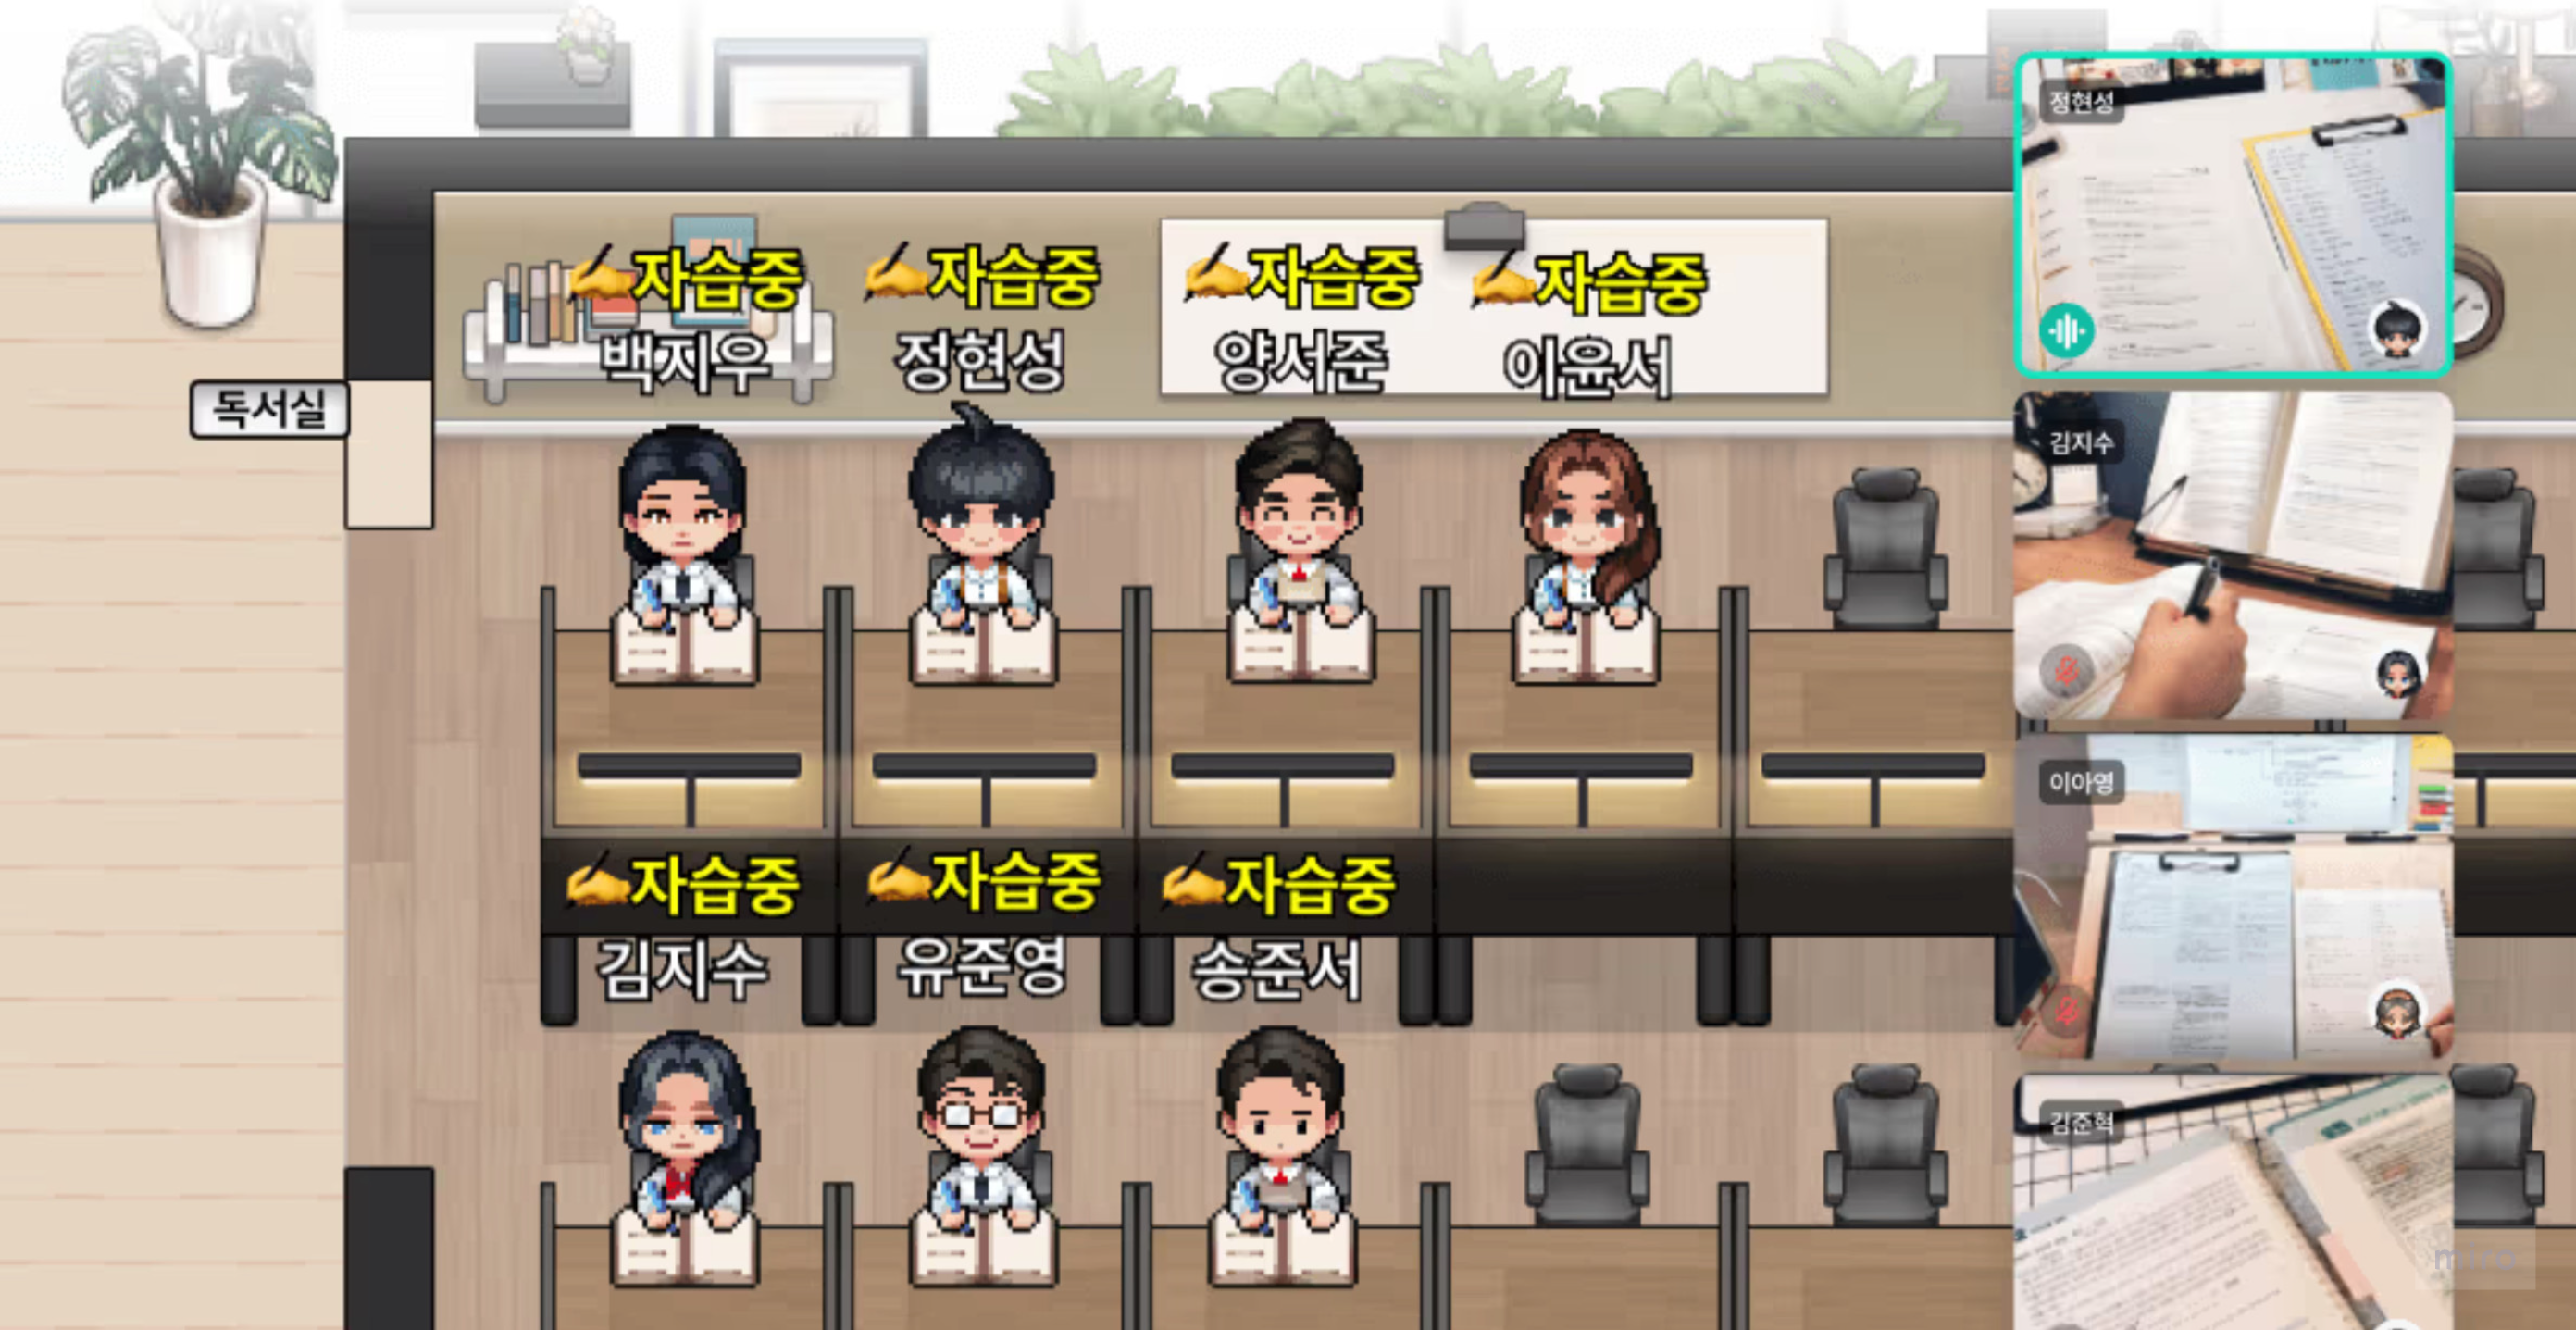
\includegraphics[width=1\linewidth]{template//images//chap4/zep_study.png}
%     \caption{zep study gathering}
%     \label{fig:placeholder}
% \end{figure}

% \subsection{경제 모델}
% 플랜은 Free / Basic / Pro / Enterprise 4종류가 있으며, 사용할 수 있는 기능의 차이가 있다.
% ZEP는 (아직) ZEPETO와 같은 앱 내 경제나 아바타 상거래 기능을 제공하지 않으며, 엔터테인먼트 중심보다는 실용성에 더 중점을 두고 있습니다.

% \begin{figure}
%     \centering
%     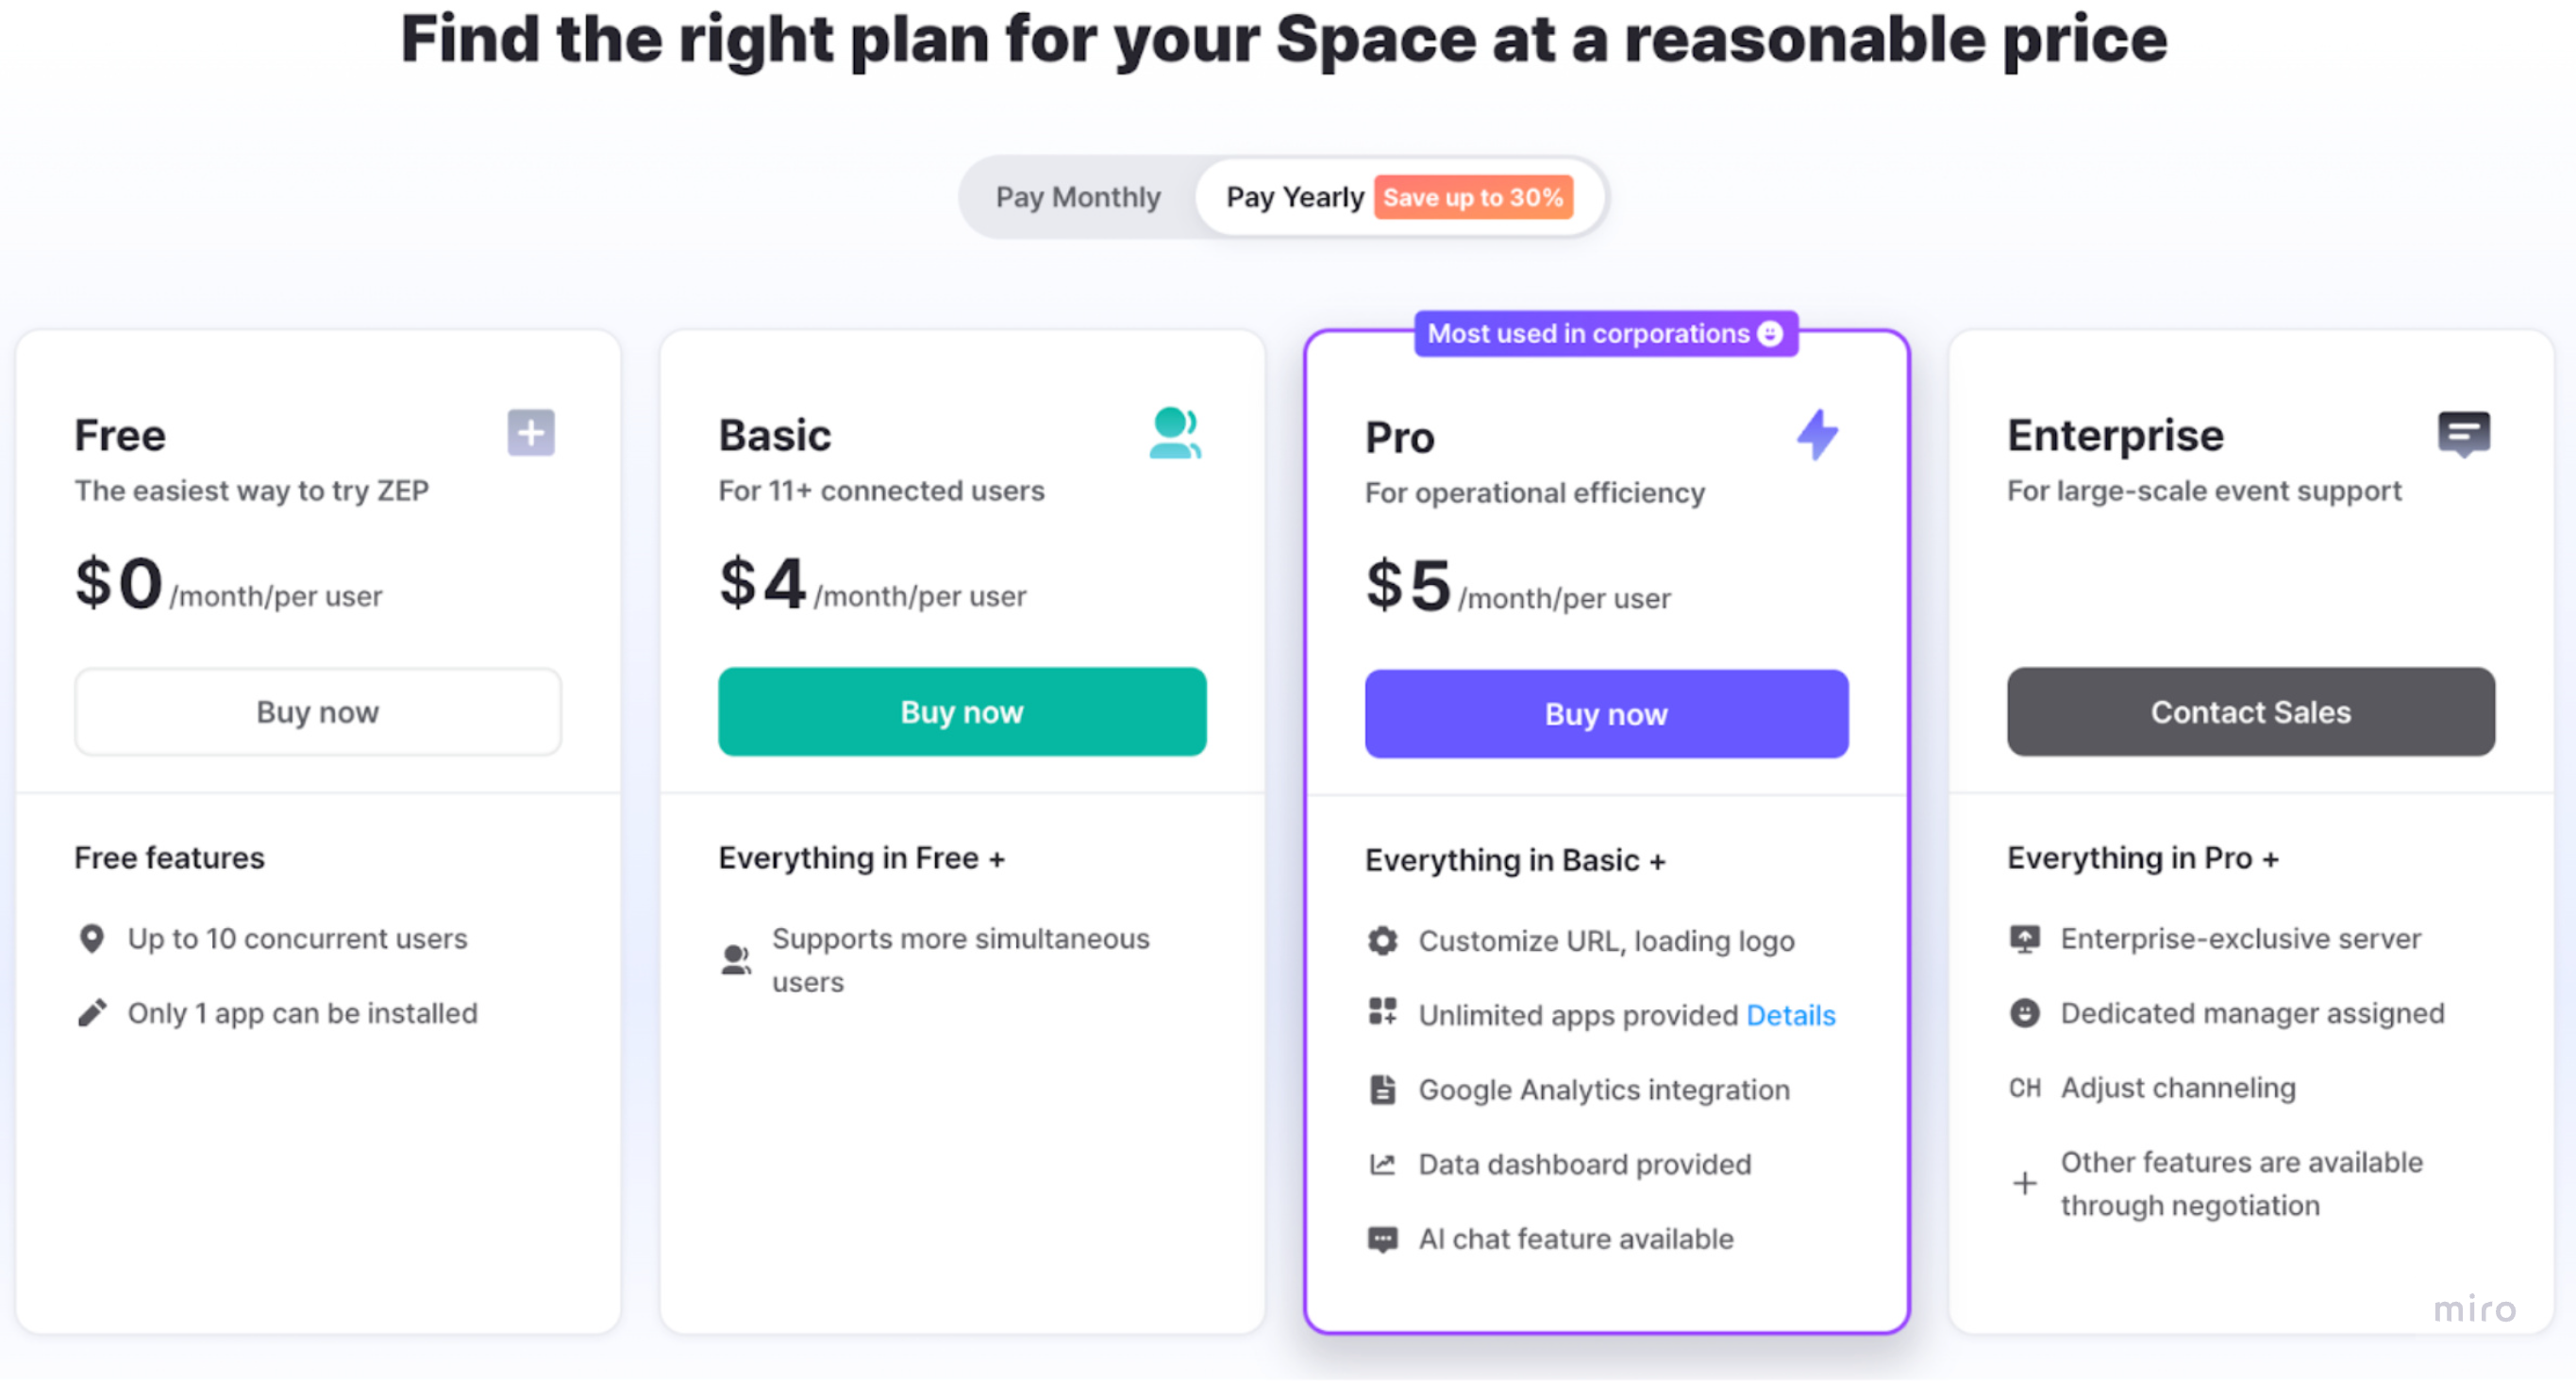
\includegraphics[width=1\linewidth]{template//images//chap4/zep_pricing.png}
%     \caption{zep pricing plan}
%     \label{fig:placeholder}
% \end{figure}

% \section{버튜버 Virtual Youtuber (VTuber)}
% 버츄얼 유튜버는 카메라나 특수 장비를 통해서 그 사람의 행동이나 표정을 대신 표현해 주는 캐릭터가 등장해 방송을 진행하는 인터넷 방송인을 말한다. 해당 분야의 선구자로 불리는 일본의 유튜버 키즈나 아이가 처음 사용하며[1] 정립된 용어다.

% \begin{figure}
%     \centering
%     \includegraphics[width=1\linewidth]{template//images//chap4/vtuber.png}
%     \caption{Vtuber}
%     \label{fig:placeholder}
% \end{figure}

% 최근 급성장한 버추얼 유튜버(VTuber) 현상은, 탈가족화된 사회에서 디지털 정체성 놀이가 어떻게 새로운 공동체적 유대와 정서적 소속감으로 확장되는지를 잘 보여준다. 버튜버는 실제 개인의 목소리와 행동을 기반으로 하지만, 시청자가 교류하는 것은 아바타 캐릭터라는 가상적 자아다. 이러한 구조는 오프라인의 ‘본래 자아’와 다른 놀이적·유동적 정체성을 무대 위에서 연기한다는 점에서, 트위터 봇 연구가 밝힌 ‘정체성 놀이’와 궤를 같이한다.
% 그러나 버튜버 팬덤은 단순히 관객적 소비에 머무르지 않는다. 팬들은 실시간 채팅, 멤버십, 슈퍼챗, 팬아트와 같은 다양한 방식으로 참여하며, 버튜버 캐릭터의 정체성과 세계를 함께 구축해간다. 이 과정에서 팬들은 서로를 알아보고 연대하며, 기존 가족이 제공하지 못하는 정서적 친밀감과 공동체적 소속을 경험한다. 이는 개인의 데이터와 감정이 모여 하나의 ‘살아 있는 네트워크’, 즉 리빙 네트워크를 형성하는 과정이다.
% 한국 사회의 맥락에서 이러한 버튜버 팬덤은, 1인 가구 증가와 가족 해체 속에서도 사람들이 여전히 소속을 갈망하고 있음을 보여준다. 즉, 버튜버라는 가상 캐릭터와의 관계는 단순한 엔터테인먼트를 넘어, 디지털 환경이 대안적 가족적 관계를 실험하는 장으로 기능한다. 이는 본 연구가 제안하는 디지털 공동체의 가능성을 뒷받침하는 중요한 사례라 할 수 있다.

% \subsection{방송 플랫폼}
% \begin{itemize}
%     \item 유튜브 : VOD, 라이브 스트리밍 플랫폼. 긴 스트리밍 지연 시간, 높은 후원 (슈퍼챗) 수수료, 시청자 채팅 관리의 어려움 때문에 한국에서는 유튜브가 라이브 스트리밍 용으로는 인기가 없으며, 주로 커버곡, 생방송 다시보기, 방송 하이라이트 편집 영상이 업로드된다.
%     \item SOOP : 라이브 스트리밍, VOD, 커뮤니티 플랫폼. 22년 이전까지 아프리카는 버츄얼에 대한 문화가 없었지만, 2022년 9월 30일 트위치의 한국 서비스 정책 변경으로 인한 반발 효과로 몇몇 버츄얼 스트리머들이 SOOP (구 아프리카TV)으로 이적하면서 버츄얼 방송이 알려졌고, 23년 트위치의 서비스 종료 발표 이후로 본격적으로 버츄얼 스트리머들이 SOOP 에서 활동을 하게 되면서 버츄얼 방송 규모가 증가했다.
%     \item 제페토 라이브 : 무료로 버츄얼 아바타를 만들고 방송할 수 있어 진입 장벽이 높지 않으며, 본인이 원하는 제스처·아이템·배경을 활용해 자신만의 연출이 가능하다. 팬이 현금화 가능한 후원 아이템을 보내 수익화할 수 있고 월 1억 원 이상의 매출을 기록하는 스트리머들도 있다고 한다. 라이브 방송 내 인터랙션 기능으로 몰입도 높고 매력적인 방송을 만들어낼 수 있으며 국내뿐만 아니라 글로벌 버튜버로서 데뷔도 가능하여 버츄얼 유튜버 지망생들이 자주 진입하는 플랫폼.
%     \item 
% \end{itemize}

% \subsection{아바타 제작}
% Live2D : 이름 그대로 2D 그래픽을 움직일 수 있게 만든다. 주로 서브컬처 창작물, 모바일 게임 등의 캐릭터 구현에 많이 쓰이고 있다.

% \section{트위터 역할극}

% 역극이란 온라인 상에서[1] 캐릭터에 이입하여 대사 및 행동 등을 연기하는 온라인 역할극을 말한다.

% \subsection{트위터봇}

% X의 API 시스템과 연동하여 시간에 맞춰 프로그램이 자동적으로 트윗을 작성하는 계정과, 사람이 직접 특정한 목적을 지니고 운영하는 정보성 계정 혹은 캐릭터 역할 놀이 계정(RPA: Role Playing Account)를 한데 아울러서 부르는 용어.

% 기본적으로 봇을 'bot'(로봇의 준말)으로 칭하게 된 것은 프로그램을 통한 게시물의 자동 작성이 로봇의 반복적인 작업을 연상시키기 때문이었지만, 한국에서 엑스 문화가 정착되며 용어의 뜻이 변화/확장된 것으로 볼 수 있다. 따라서 목적에 따른 분류도 가능한데, 주로 정보전달을 목적으로 한 계정을 정보봇이라 부르고 특정 캐릭터가 엑스를 한다는 컨셉을 잡은 계정을 캐릭터봇이라고 부른다. 원작자의 공인을 받거나 원작의 권리자가 직접 운영하는 봇을 공식봇이라고 부르기도 하나 실제로 이는 굉장히 드문 사례이므로 대다수의 봇은 비공식의 영역에 속해 있으며, 특히 캐릭터봇은 2차 창작의 일종으로 분류할 수도 있다.

% \subsection{캐릭터봇}
% X의 사적 활용, 즉 개인의 소소한 일을 쓰는 마이크로블로그의 성격에 주목하여 '가상의 인물이 X를 사용하는 것을 가정한 연출'을 하는 경우도 있다. 이것을 흔히 캐릭터봇이라 한다. 그 특성상 만화, 애니메이션, 게임의 등장인물이 주로 선택된다.

% 만화/애니메이션이 크게 발달한 일본에서는 이와 같은 가상의 캐릭터를 연출하는 X 계정이 상당히 빠르게 만들어졌으나, 자동 게시물과 자동 답변을 사용하는 계정만을 bot으로 칭하고, 사람이 직접 게시물을 쓰며 의도적인 연출을 하는 계정은 주로 '흉내내기 계정'이라 부른다. 한국에서는 대체로 '봇'이라는 용어 아래 서로가 혼재되어 있는 상황이며, 편의상 '자동봇 / 수동봇'이라는 식으로 나누는 경우가 많다. 다만 봇(bot)이라는 단어 자체가 자동으로(auto) 운영된다는 의미를 내포하기 때문에 '수동봇'이라는 표현은 엄밀히 말하면 올바르다고 볼 수 없다, 이 때문에 일부 캐릭터봇은 RPA(Role-Playing Account: 역할놀이 계정)라는 이름을 사용하고 있다.

% 캐릭터봇은 대부분 특정 작품의 팬들이 자발적으로 만든다. 캐릭터봇을 만드는 이유는 다양할 수 있다. 'X에서 해당 캐릭터가 게시하는 것을 보고 싶다' 부터,, 직접 게시하며 캐릭터를 연출해 '캐릭터가 된 기분을 느끼기 위해', 드물게는 '캐릭터에 대한 특별한 애정/사연 이 있어서'[2] 이 있거나, 등등 여러 이유가 있을 수 있다.

% 한국의 캐릭터봇은 대다수가 캐릭터가 된 기분을 느끼기 위한 흉내내기 용도에 가깝다. 캐릭터봇을 통해 해당 캐릭터의 팬과 대화를 나누며 자신이 좋아하는 캐릭터를 남들 또한 좋아해 준다는 것을 체감하고, 해당 캐릭터에 이입함으로써 '자신이 타인에게 사랑받는 것 같은' 대리만족적인 위안감을 얻는 경우다. 이는 인터넷상에서의 페르소나가 좀 더 구체적으로 튀어나온 것이라고 해석할 수 있다.

% 이를 위해 캐릭터봇은 소위 '선점효과'를 노린 계정 개설 경쟁이 심심찮게 벌어진다. 예를 들어 애니메이션의 신 캐릭터나 게임에서의 신규 직업군 업데이트 소식이 나오자마자 공식 설정이나 게임 내의 묘사가 제대로 공개되지도 않은 상태에서 소위 말하는 '원조 봇' 타이틀 선점을 위해 무분별하게 계정부터 만드는 경우이다.[3]


% [관련 논문]
% 소셜네트워크와 정체성 놀이: 트위터 봇 사례연구를 중심으로

% 윤명희와 손수빈(2015)의 트위터 봇 연구는, 디지털 상호작용이 단순한 자동화가 아니라 쌍방향적 정체성 놀이임을 보여준다. 봇 관리자와 팔로워는 서로의 ‘세계관’을 공유하고, 캐릭터 변형(캐변)과 몰입을 통해 놀이적 친밀성을 만들어낸다. 이러한 관계는 혈연이나 제도적 소속이 아닌, 놀이와 상상력 위에서 형성된 새로운 형태의 사회적 유대다. 이는 본 연구에서 탐구하는 리빙 네트워크—탈가족화된 한국 사회에서, 감정적·디지털적 흔적들이 살아 있는 공동체적 유기체로 진화하는 과정—와 직접적으로 맞닿아 있다. 즉, 디지털 공간은 단순한 소통 플랫폼을 넘어, 새로운 가족적 관계를 모색하는 실험장으로 기능한다.

% 1. 정체성 놀이 → 새로운 소속감
% 트위터 봇 논문: 캐릭터를 연기하며 팔로워와 상호작용 → 놀이가 단순한 가면이 아니라 정서적 친밀감을 낳음.
% 네 논문: MBTI 채팅, 게임, 디지털 유대 → 놀이적 자아 실험이 대안적 가족/공동체로 확장 가능.

% 즉, 정체성 놀이가 단순한 퍼포먼스가 아니라 새로운 ‘관계 맺기’의 토대라는 점을 강조할 수 있음.


% 2. 쌍방향성 → 살아 있는 네트워크
% 트위터 봇: 팔로워는 관객이 아니라 참여자, 캐릭터 변화를 함께 만들어감.
% 네 논문: 데이터, 루틴, 감정 흔적이 서로 얽히며 유기적이고 살아 있는 네트워크를 생성.
% 봇 연구의 쌍방향적 구조를 네가 제안하는 ‘리빙 네트워크’의 사회적 사례로 활용 가능.


% 3. 탈가족화 맥락과 한국 사회
% 트위터 봇 논문도 참여자가 대부분 젊은 20대, 개인주의적 상황에서 정서적 친밀감을 디지털에서 찾음.
% 네 논문은 이를 한국 사회의 가족 구조 해체, 1인 가구 증가라는 더 큰 맥락과 연결.
% 봇 연구 = 미시적 사례, 네 논문 = 거시적 구조 → 서로 보완 가능.


% 4. 시적·유기적 은유와의 접점
% 트위터 봇 논문은 ‘세계관’을 공유하고 그 안에서 정체성을 연기함.
% 네 논문은 웹을 **“살아 있는 생태계, 서정적 서식지”**로 상상.
% 둘 다 기술적 환경을 정서적·문화적 공간으로 재해석한다는 점에서 호환됨.


